% Created 2021-04-25 Sun 17:26
% Intended LaTeX compiler: pdflatex

\documentclass[a4paper,12pt]{article}
\usepackage[margin=2cm]{geometry}

\usepackage{hyperref}
\usepackage[utf8]{inputenc}
\usepackage{fixltx2e}
\usepackage{graphicx}
\usepackage{longtable}
\usepackage{float}
\usepackage{wrapfig}
\usepackage{rotating}
\usepackage[normalem]{ulem}
\usepackage{amsmath}
\usepackage{textcomp}
\usepackage{marvosym}
\usepackage{wasysym}
\usepackage{multicol}
\usepackage{amssymb}
\tolerance=1000
\usepackage{listings}
\usepackage{titlesec}
\newcommand{\sectionbreak}{\clearpage}
\usepackage[scaled]{helvet}
\usepackage{courier}
\linespread{1.10}
\usepackage[margin=1.0in]{geometry}
\usepackage[numbers,sort&compress,square]{natbib}
\usepackage{glossaries}
\makeglossaries
\usepackage{setspace} \singlespacing
\usepackage{enumitem}
\setlist[itemize]{noitemsep, topsep=0pt}
\setlist[enumerate]{noitemsep, topsep=0pt}
\setlength\arrayrulewidth{0.7pt} % width of table line
\usepackage[english]{babel}
\addto\captionsenglish{\renewcommand\contentsname{Outline}}
\hypersetup{linktoc = all, colorlinks = true, urlcolor = DodgerBlue4, citecolor = PaleGreen1, linkcolor = black}
\usepackage[UTF8, heading]{ctex}
\usepackage{xltxtra}
\usepackage{xeCJK}
\usepackage{lmodern}
\usepackage{verbatim}
\usepackage{float}
\usepackage{tikz}
\usepackage{wrapfig}
\usepackage{soul}
\usepackage{textcomp}
\usepackage{algorithm}
\usepackage{algorithmic}
\usepackage{marvosym}
\usepackage{wasysym}
\usepackage{natbib}
\usepackage{fancyhdr}
\usepackage{fontspec,xunicode,xltxtra}
\usepackage{CJKnumb}
\usepackage{amsfonts}
\usepackage[default]{sourcecodepro}
\usepackage[T1]{fontenc}
\setCJKmainfont{SimSun} % 設置缺省中文字體
\setmainfont[Scale=0.8]{Times New Roman} % 英文襯線字體
\setsansfont[Scale=0.8]{Source Code Pro} % 英文無襯線字體
\setmonofont[Scale=0.8]{Source Code Pro} % 英文等寬字體
\setCJKmainfont[Scale=0.9]{Adobe Heiti Std} % 中文字體
\setCJKmonofont[Scale=0.9]{Adobe Heiti Std}
\usepackage{color}
\RequirePackage{fancyvrb}
\usepackage{placeins}
\hypersetup{pdfauthor={Name}}
\definecolor{dkgreen}{rgb}{0,0.6,0}
\definecolor{dred}{rgb}{0.545,0,0}
\definecolor{dblue}{rgb}{0,0,0.545}
\definecolor{lgrey}{rgb}{0.9,0.9,0.9}
\definecolor{gray}{rgb}{0.4,0.4,0.4}
\definecolor{darkblue}{rgb}{0.0,0.0,0.6}
\definecolor{bubbles}{rgb}{0.91, 1.0, 1.0}
\definecolor{foreground}{RGB}{220,220,204} % 淺灰
\definecolor{background}{RGB}{62,62,62} % 淺黑
\definecolor{preprocess}{RGB}{250,187,249} % 淺紫
\definecolor{var}{RGB}{239,224,174} % 淺肉色
\definecolor{string}{RGB}{154,150,230} % 淺紫色
\definecolor{type}{RGB}{225,225,116} % 淺黃
\definecolor{function}{RGB}{140,206,211} % 淺天藍
\definecolor{keyword}{RGB}{239,224,174} % 淺肉色
\definecolor{comment}{RGB}{180,98,4} % 深褐色
\definecolor{doc}{RGB}{175,215,175} % 淺鉛綠
\definecolor{comdil}{RGB}{111,128,111} % 深灰
\definecolor{constant}{RGB}{220,162,170} % 粉紅
\lstdefinelanguage{cpp}{ %%定義語言style
backgroundcolor=\color{bubbles},
basicstyle=\footnotesize \ttfamily \color{dblue},
breakatwhitespace=false,
breaklines=true,
captionpos=b,
comment=[l]{\#},
morecomment=[s]{/*}{*/},
commentstyle=\color{comment} \slshape \small \itshape,
ndkeywords={print, printf, repeat, struct, enum, case, switch, func, let, var, boolean, throw, import, typeof, null, catch, switch, for, in, int, str, float, self, return, class, if ,elif, endif, while, do, else, True, False , catch, def},
ndkeywordstyle=\color{dred} \bfseries \small \mono,
identifierstyle=\color{black},
deletekeywords={...},
escapeinside={\%*}{*)},
frame=single,
frameround=tttt,
framesep=0pt,
rulecolor=\color{background},
morekeywords={BRIEFDescriptorConfig,string,TiXmlNode,DetectorDescriptorConfigContainer,istringstream,cerr,exit},
identifierstyle=\color{black},
stringstyle=\color{blue},
rulecolor=\color{black},
showspaces=false,
showstringspaces=false,
showtabs=true,
stepnumber=1,
tabsize=5,
title=\lstname,
}
\lstdefinelanguage{shell}{
backgroundcolor=\color{keyword},
basicstyle=\footnotesize \ttfamily \color{dblue} \small \mono \bfseries,
breakatwhitespace=false,
breaklines=true,
captionpos=b,
comment=[l]{\#},
morecomment=[s]{/*}{*/},
commentstyle=\color{comment} \slshape \small \itshape,
identifierstyle=\color{black},
deletekeywords={...},
escapeinside={\%*}{*)},
frame=single,
frameround=tttt,
framesep=0pt,
rulecolor=\color{background},
morekeywords={BRIEFDescriptorConfig,string,TiXmlNode,DetectorDescriptorConfigContainer,istringstream,cerr,exit},
identifierstyle=\color{black},
stringstyle=\color{blue},
rulecolor=\color{black},
showspaces=false,
showstringspaces=false,
showtabs=false,
stepnumber=1,
tabsize=5,
title=\lstname,
}
\author{Yung Chin, Yen}
\date{\today}
\title{Advanced Swift Ui}
\begin{document}

\maketitle
\tableofcontents

\newpage

\section{MVVM}
\label{SW-MVVM}
\subsection{Design pattern}
\label{sec:orgdee0494}
MVVM 的概念最早應該是在 2005 年由 Microsoft的\href{https://blogs.msdn.microsoft.com/johngossman/2005/10/08/introduction-to-modelviewviewmodel-pattern-for-building-wpf-apps/}{John Gossman}提出來的,它的概念是,整個 Swift project 會拆分成三個部份: View、ViewModel、Model,其中 View 的角色就是單純的視覺元件,像是按鈕、文字標籤等等,在 View 裡面不會有邏輯、狀態等等,單純就是個呈現資料的元件。而要讓 View 呈現資料,最直覺的方式,就是把 View 跟 Model 做綁定,讓 View 的元件跟著 Model 一起做變化。但這樣會有個問題,就是通常 Model 來的資料,並不是簡單就能轉換成 View 的樣式的,這時候就需要有個物件,介在 View 跟 Model 的中間,這個物件會掌管這些跟 View 高度相關的邏輯的操作,像是轉換 Date 物件變成人看得懂的文字格式等,稱之為 ViewModel。上面的概念可以畫成這樣的資料流:\\

\begin{figure}[htbp]
\centering
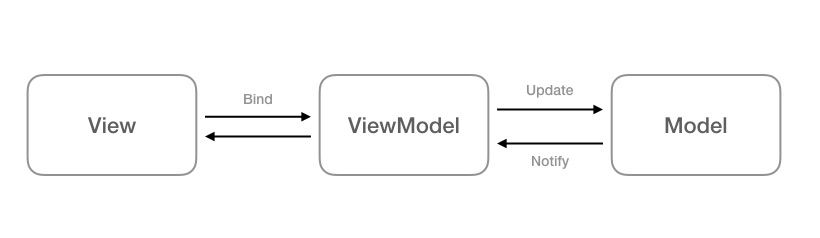
\includegraphics[width=500]{images/MVVM-Basic.jpg}
\caption{\label{fig: MVVMPNG}MVVM Architecture}
\end{figure}

在 iOS 開發上,依照上述 MVVM 的定義,ContentView 變成一個單純的 View,而我們會另外產生一個 ViewModel 來負責 presentational logic 跟部份的 controller logic。所以在View裡面,就只會有:\\
\begin{enumerate}
\item View logic,所有跟呈現有關的 Code\\
\item 綁定 ViewModel\\
\end{enumerate}
而在 ViewModel 裡面,則是負責兩個部份:\\
\begin{enumerate}
\item Controller logic,如 pagination, error handling,… etc\\
\item Presentation logic,提供接口讓 View 綁定(binding)(提供適合在View中呈現的資料)\\
\end{enumerate}
開發上,一旦 View 綁定好 ViewModel 的資料,在撰寫商業邏輯的時候,就可以不用管包括動畫、轉場、main thread 等等跟 View 相關的問題,因為分工明確所以就不會有寫起來綁手綁腳的感覺。更棒的是,並且因為 ViewModel 是一個單純的、沒有相依於 View 的物件,所以要做測試簡單多了!\\
\href{https://www.codementor.io/@koromiko/mvvm-app-cl1wvw2sh}{資料來源: 歡迎來到真實世界 - 原來是那個傳說中的MVVM阿}\\
\subsection{What is the idea behind MVVM}
\label{sec:org0fa99d4}
\begin{enumerate}
\item Model
\label{sec:org242105f}
\begin{itemize}
\item Business logic\\
\item UI Independent\\
\end{itemize}
\item View
\label{sec:org1c7efd4}
\begin{itemize}
\item Presentation\\
\item User interaction\\
\end{itemize}
\item ViewModel
\label{sec:orga653343}
\begin{itemize}
\item Presentation logic\\
\item Glue between Model and View\\
\end{itemize}
\item 為什麼要拆成三部份(What does it solve?)
\label{sec:orgef4b9a5}
\begin{itemize}
\item MVC - Massive View Controller\\
\item Testability\\
\item Code organization\\
\item Code reusability\\
\end{itemize}
\item Limitations / Cons
\label{sec:org585ad1b}
\begin{itemize}
\item Requires binding\\
\item Potential for boilerplate code\\
\item Overkill for simple views and logic\\
\item Doesn't cover every case\\
\end{itemize}
\end{enumerate}
\subsection{DEMO}
\label{sec:orgae1834c}
以``推薦書單''的 APP 為例:\\
\begin{itemize}
\item Model: 包含書名、作者、出版社\ldots{}.,而實際的資料來源可能是雲端資料庫(Firebase)、Web API、本機資料庫(Core data)。\\
\lstset{breaklines=true,language=swift,label= ,caption= ,captionpos=b,firstnumber=1,numbers=left}
\begin{lstlisting}
struct Book {
    let title: String
    let author: String
    let dateReleased: String
    let publishCamp: String
    let publishCity: String
    let isFavorite: Bool
}
\end{lstlisting}
\item View: 在 APP 畫面上呈現 Model 中資料的元件,如 Text, Image, Button, List\ldots{}..\\
\item ViewModel: 將 Model 中的資料取出,供 View 呈現,或是接受 View 輸入的資料,存回 Model。以``推薦書單 APP''為例,其 ViewModel 可能包含如下 struct:\\
\lstset{breaklines=true,language=swift,label= ,caption= ,captionpos=b,firstnumber=1,numbers=left}
\begin{lstlisting}
struct BookDetailViewModel {
    var book: Book

    var isFavorite: Bool

    init(book: Book) {
        self.book = book
        self.isFavorite = false
    }

    var title: String {
        return self.book.title
    }

    var author: String {
        return self.book.author
    }

    var dateReleased: String {
        return self.book.dateReleased
    }

    // 呈現時要求以 遠流出版社(台北市) 的格式來呈現
    var publisher: String {
        let output = self.book.publishCamp + "(" + self.book.publishCity + ")"
        return output
    }
}
\end{lstlisting}
從 Model 中可以看到書籍的記錄欄位只有``出版社''(publishCamp)和``出版地點''(publishCity),但若 app 對顯示結果的格式要求為``出版社(出版地點)'',則可以在 ViewModel 中來處理。\\
此外,如果在 View 上有一個 Favorite Button,則當 user 點了 Favorite 後,ViewModel 應負責將 struct 中的 isFavorite 改存 True,並回存至 Model 中。Model 的資料只能透過 ViewModel 來新增刪除,View 無法直接染指。\\
Model 與 UI 完全無關,單純用來儲存資料,ViewModel 為 Model 與 View 溝通的橋樑。\\
\end{itemize}
\subsection{Model 要用 Struct 或是 Class}
\label{sec:org7ad1a31}
\href{https://www.appcoda.com.tw/swift-class/}{資料來源:Swift Class vs Struct:設計 Model 時,該用 Struct 還是 Class 呢?}\\
\begin{enumerate}
\item Struct 與 Class 的不同性質
\label{sec:org44bee36}
首先,當我們指派 (assign) 一個實體給一個辨識符(identifier,也就是變數/常數名)的時候,如果該實體是 struct 的話,該辨識符所容納的會是該實體的所有內容;但如果它是 class 的話,這個辨識符就只會容納存放該實體的位址:\\
\lstset{breaklines=true,language=swift,label= ,caption= ,captionpos=b,firstnumber=1,numbers=left}
\begin{lstlisting}
// 用 struct 定義 Dog。
struct Dog {
    var name = "Bart"
}
// 整個 Dog 實體都會被存到 myDog 裡。
var myDog = Dog()
// 用 class 定義 Cat。
class Cat {
    var name = "Mimi"
}
// myCat 只會儲存 Cat 實體的位址。Cat 實體本身會被存到別的地方。
var myCat = Cat()
\end{lstlisting}
也就是說,當我們使用辨識符的時候,如果它的型別是 struct 的話,我們在操作的實體都會是本地的。但是當我們在操作 class 型別的辨識符的話,那麼我們實際上是透過辨識符在操作一個遠端的實體。所以,當我們更改這些實體的屬性的時候,它們的行為就不太一樣了:\\
\lstset{breaklines=true,language=swift,label= ,caption= ,captionpos=b,firstnumber=1,numbers=left}
\begin{lstlisting}
// 使用 struct。
var herDog = Dog() {
    // 如果 herDog 有變動的話就顯示訊息。
    didSet {
        print("Her dog is changed!")
    }
}
herDog.name = "Starlord"
// Her dog is changed!
// 使用 class。
var herCat = Cat() {
    didSet {
        print("Her cat is changed!")
    }
}
herCat.name = "Mumu"
// 沒有訊息。
\end{lstlisting}
怎麼會有這樣的差別呢?因為 herDog 儲存了所有的 Dog 實體內容,所以任何 Dog 實體的屬性的變動,就等於說 herDog 本身有變動。然而,herCat 並沒有儲存 Cat 實體的內容,所以 Cat 實體屬性的變動是在別的地方發生的,且 herCat 本身所儲存的 Cat 實體位址並沒有任何的改變。\\
由圖\ref{fig: MVVMPNG}可看出,\\
\item MVVM 中的 Model
\label{sec:orgb5034cf}
\end{enumerate}
\subsection{DICE DEMO}
\label{sec:orgabde78a}
\subsection{Further Reading Resources}
\label{sec:org61d1971}
\begin{itemize}
\item \href{https://www.youtube.com/watch?v=1IlUBHvgY8Q\&t=29s}{SwiftUI MVVM Programming with ObservableObject @Published @ObservedObject}\\
\item \href{https://www.youtube.com/watch?v=LntH6moCuo0}{SwiftUI 2.0: MVVM - A Practical Approach}\\
\item \href{https://www.youtube.com/watch?v=gkAV4D1nopA}{SwiftUI Tip Calculator Using MVVM Design Pattern}\\
\item \href{https://www.youtube.com/watch?v=cbqMkIG6Qeg}{Understanding MVVM Design Pattern}: 講的超清楚\\
\item Video: \href{https://www.youtube.com/watch?v=EhtK\_H9LsYQ}{MVVM SwiftUI - Model View ViewModel Pattern - Getting Started}\\
\item Video: \url{https://www.youtube.com/watch?v=LntH6moCuo0}\\
\item Video: \href{https://www.youtube.com/watch?v=sWx8TtRBOfk}{MVVM in Practice - RWDevCon Session - raywenderlich.com}\\
\item GitHub: \url{https://github.com/rebeloper/SwiftUIMVVM.git}\\
\end{itemize}
\newpage

\section{Review}
\label{SW-Review}
\begin{itemize}
\item Functions: Tasks management project: task listing, adding, removing, editing\\
\item Technoloties: View navigation, variable sharing, data model\\
\end{itemize}
參考資料: \href{https://medium.com/better-programming/replicating-the-ios-reminders-app-part1-44211a7b7029}{Building a To-Do List App with SwiftUI, Combine, and Firebase}\\
\subsection{Data Model}
\label{sec:orgc259d2c}
\lstset{breaklines=true,language=swift,label= ,caption= ,captionpos=b,numbers=none}
\begin{lstlisting}
//
//  Task.swift
//  taskManagement
//
//  Created by yen yung chin on 2021/2/18.
//

import Foundation


struct Task: Identifiable {
    var id = UUID()
    var title: String
    var completed: Bool
}

#if DEBUG
let testDataTasks = [
    Task(title: "Implement UI", completed: true),
    Task(title: "Share data", completed: false),
    Task(title: "Create Chart", completed: false),
    Task(title: "Connect to Firebase", completed: false),
    Task(title: "PROFIT!!!", completed: false)
]
#endif
\end{lstlisting}
\subsection{Basic UI}
\label{sec:org10d8b2c}
\begin{enumerate}
\item Change struct name (ContentView.swift)
\label{sec:org0f3a882}
\begin{enumerate}
\item right click on struct ContentView\\
\item Refactor\\
\item Rename\ldots{}: to \textbf{TaskListView}\\
\item The file name on navigator (left panel in Xcode) will be renamed to \textbf{TaskListView.swift}\\
\end{enumerate}
\item classify files into the following group
\label{sec:org959063e}
\begin{itemize}
\item App\\
\item View\\
\item Model\\
\end{itemize}
\begin{center}
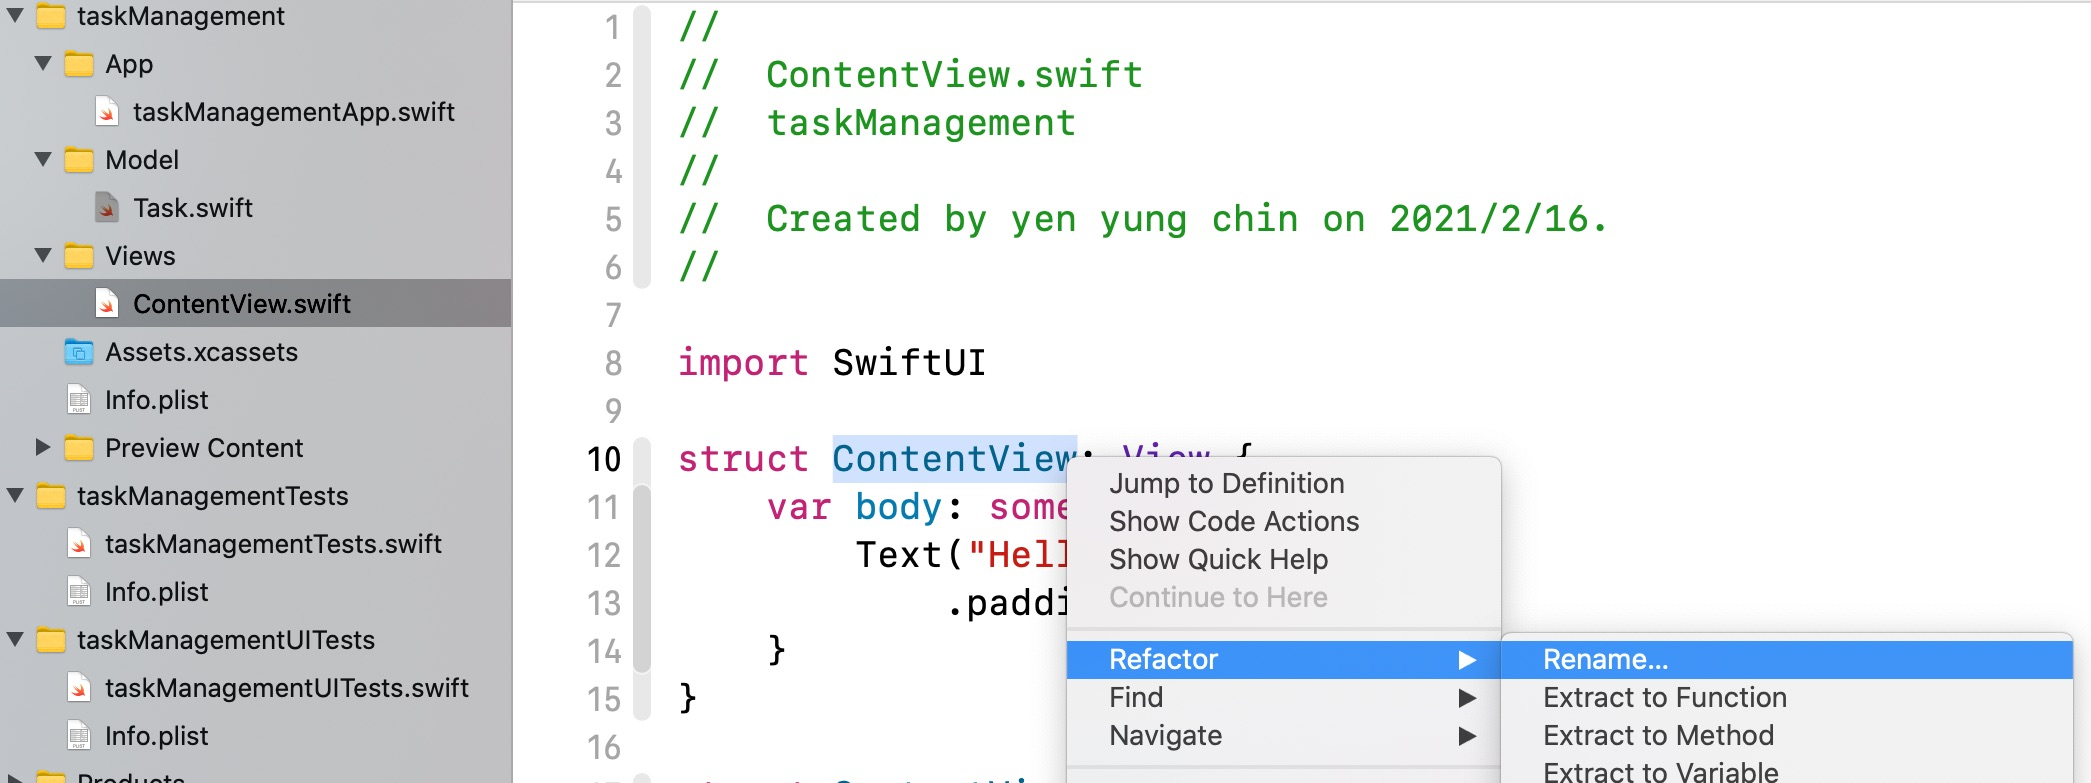
\includegraphics[width=400]{images/renameStruct.jpg}
\label{fig:RenameStructName}
\end{center}
\item Create basic UI
\label{sec:org1ad7d2c}
\begin{enumerate}
\item TaskListView.swift
\label{sec:org78e3b4a}
\lstset{breaklines=true,language=swift,label= ,caption= ,captionpos=b,firstnumber=1,numbers=left}
\begin{lstlisting}
//
//  ContentView.swift
//  taskManagement
//
//  Created by yen yung chin on 2021/2/16.
//

import SwiftUI

struct TaskListView: View {
    let tasks = testDataTasks
    var body: some View {
        NavigationView {
            VStack(alignment: .leading, spacing: 10, content: {
                List(tasks) { task in
                    Image(systemName: "circle")
                    Text(task.title)
                }
                HStack(alignment: .center, spacing: 10, content: {
                    Image(systemName: "plus.circle.fill")
                    Text("New Task")
                }).padding()

            }).navigationTitle("Tasks")
        }
    }
}

struct ContentView_Previews: PreviewProvider {
    static var previews: some View {
        TaskListView()
    }
}

\end{lstlisting}
\item Extract the task cell
\label{sec:org91adb46}
\begin{enumerate}
\item Grouping the Image and Text with HStack\\
\item cmd+click Htack\\
\item Extract SubView\\
\item Fix the compile error(inject needed variable)\\
\end{enumerate}
\lstset{breaklines=true,language=swift,label= ,caption= ,captionpos=b,firstnumber=1,numbers=left}
\begin{lstlisting}
//
//  ContentView.swift
//  taskManagement
//
//  Created by yen yung chin on 2021/2/16.
//

import SwiftUI

struct TaskListView: View {
    let tasks = testDataTasks
    var body: some View {
        NavigationView {
            VStack(alignment: .leading, spacing: 10, content: {
                List(tasks) { task in
                    TaskCell(task: task)
                }
                HStack(alignment: .center, spacing: 10, content: {
                    Image(systemName: "plus.circle.fill")
                    Text("New Task")
                }).padding()

            }).navigationTitle("Tasks")
        }
    }
}

struct ContentView_Previews: PreviewProvider {
    static var previews: some View {
        TaskListView()
    }
}

struct TaskCell: View {
    var task: Task
    var body: some View {
        HStack {
            Image(systemName: "circle")
            Text(task.title)
        }
    }
}

\end{lstlisting}
\end{enumerate}
\end{enumerate}
\subsection{MVVM}
\label{sec:org454c953}
以MVVM架構來開發project\\
\begin{enumerate}
\item ViewModel
\label{sec:org38479bb}
\begin{enumerate}
\item Diagram for now
\label{sec:org05c86c8}
\begin{center}
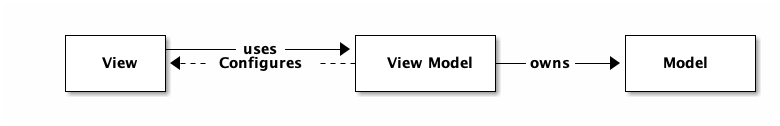
\includegraphics[width=.9\linewidth]{images/mvvm-d1.png}
\end{center}

\item Model for the future
\label{sec:org9759b37}
\begin{center}
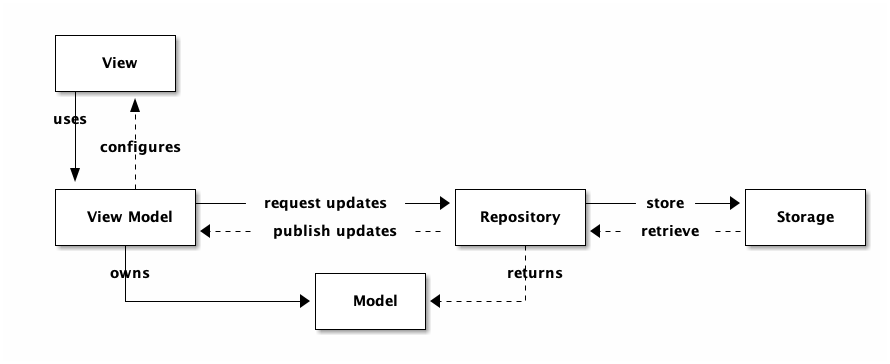
\includegraphics[width=.9\linewidth]{images/mvvm-d2.png}
\end{center}

\item TaskCellViewModel
\label{sec:org7a26d83}
\lstset{breaklines=true,language=swift,label= ,caption= ,captionpos=b,firstnumber=1,numbers=left}
\begin{lstlisting}
//
//  TaskCellViewModel.swift
//  taskManagement
//
//  Created by yen yung chin on 2021/2/20.
//

import Foundation
import Combine

class TaskCellViewModel: ObservableObject, Identifiable  {
    @Published var task: Task

    @Published var completionStateIconName = ""
    private var cancellables = Set<AnyCancellable>()
    init(task: Task) {
        self.task = task
        $task
            .map { task in
                return task.completed ? "checkmark.circle.fill" : "circle"
            }
            .assign(to: \.completionStateIconName, on: self)
            .store(in: &cancellables)
    }
}

\end{lstlisting}
\item TaskListViewModel
\label{sec:org1698a7d}
\lstset{breaklines=true,language=swift,label= ,caption= ,captionpos=b,firstnumber=1,numbers=left}
\begin{lstlisting}
//
//  TaskListViewModel.swift
//  taskManagement
//
//  Created by yen yung chin on 2021/2/20.
//

import Foundation
import Combine

class TaskListMiewModel: ObservableObject {
    @Published var taskCellViewModels = [TaskCellViewModel]()

    init() {
        self.taskCellViewModels = testDataTasks.map { task in
            TaskCellViewModel(task: task)
        }
    }

}

\end{lstlisting}
\end{enumerate}
\item View
\label{sec:orge9e8731}
TaskListView.swift\\
\lstset{breaklines=true,language=swift,label= ,caption= ,captionpos=b,firstnumber=1,numbers=left}
\begin{lstlisting}
//
//  ContentView.swift
//  taskManagement
//
//  Created by yen yung chin on 2021/2/16.
//

import SwiftUI

struct TaskListView: View {
    @ObservedObject var taskListVM = TaskListMiewModel()

    var body: some View {
        NavigationView {
            VStack(alignment: .leading, spacing: 10, content: {
                List(taskListVM.taskCellViewModels) { task in
                    TaskCell(taskCellVM: task)
                }
                HStack(alignment: .center, spacing: 10, content: {
                    Image(systemName: "plus.circle.fill")
                    Text("New Task")
                }).padding()

            }).navigationTitle("Tasks")
        }
    }
}

struct ContentView_Previews: PreviewProvider {
    static var previews: some View {
        TaskListView()
    }
}

struct TaskCell: View {
    @ObservedObject var taskCellVM: TaskCellViewModel

    var body: some View {
        HStack {
            Image(systemName: taskCellVM.completionStateIconName)
            Text(taskCellVM.task.title)
        }
    }
}

\end{lstlisting}
\end{enumerate}
\subsection{New task}
\label{sec:orgd87a94c}
加入新增task功能,真正的新增功能由ViewModel實作,View負責界面及呼叫該功能\\
\begin{enumerate}
\item View
\label{sec:orgb178fa2}
\begin{enumerate}
\item NewTaskView.swift
\label{sec:orgda00a9e}
\lstset{breaklines=true,language=swift,label= ,caption= ,captionpos=b,firstnumber=1,numbers=left}
\begin{lstlisting}
//
//  NewTaskView.swift
//  taskManagement
//
//  Created by yen yung chin on 2021/2/20.
//

import SwiftUI

struct NewTaskView: View {
    @ObservedObject var taskListVM = TaskListMiewModel()
    @State var taskTitle: String = ""

    @Environment(\.presentationMode) var presentation

    var body: some View {
        VStack {
            Text("New Task")
                .font(.largeTitle)
            TextField("Enter task name", text: self.$taskTitle)
            Button(action: {
                taskListVM.addTask(task: Task(title: self.taskTitle, completed: false))
                self.presentation.wrappedValue.dismiss()
            }, label: {
                Text("Done")
            })
            Spacer()
        }.padding()
    }
}

struct NewTaskView_Previews: PreviewProvider {
    static var previews: some View {
        NewTaskView()
    }
}

\end{lstlisting}
\item TaskListView.swift
\label{sec:org3150e32}
\lstset{breaklines=true,language=swift,label= ,caption= ,captionpos=b,firstnumber=1,numbers=left}
\begin{lstlisting}
//
//  ContentView.swift
//  taskManagement
//
//  Created by yen yung chin on 2021/2/16.
//

import SwiftUI

struct TaskListView: View {
    @ObservedObject var taskListVM = TaskListMiewModel()
    var body: some View {
        NavigationView {
            VStack(alignment: .leading, spacing: 10, content: {
                List(taskListVM.taskCellViewModels) { task in
                    TaskCell(taskCellVM: task)
                }


                HStack(alignment: .center, spacing: 10, content: {
                    Image(systemName: "plus.circle.fill")
                    Button(action: /*@START_MENU_TOKEN@*/{}/*@END_MENU_TOKEN@*/, label: {
                        /*@START_MENU_TOKEN@*/Text("Button")/*@END_MENU_TOKEN@*/
                    })
                    Text("New Task")
                }).padding()

                .navigationBarTitle("Tasks", displayMode: .inline)

                .navigationBarItems(trailing: NavigationLink(
                                        destination: NewTaskView(taskListVM: taskListVM, taskTitle: ""),
                                        label: {
                                            Text("New Task")
                                        }))

            })
        }
    }
}

struct ContentView_Previews: PreviewProvider {
    static var previews: some View {
        TaskListView()
    }
}

struct TaskCell: View {
    @ObservedObject var taskCellVM: TaskCellViewModel

    var body: some View {
        HStack {
            Image(systemName: taskCellVM.completionStateIconName)
            Text(taskCellVM.task.title)
        }
    }
}

\end{lstlisting}
\end{enumerate}
\item ViewModel
\label{sec:org25c5da1}
\begin{enumerate}
\item TaskListViewModel.swift
\label{sec:org6dac5da}
\lstset{breaklines=true,language=swift,label= ,caption= ,captionpos=b,firstnumber=1,numbers=left}
\begin{lstlisting}
//
//  TaskListViewModel.swift
//  taskManagement
//
//  Created by yen yung chin on 2021/2/20.
//

import Foundation
import Combine

class TaskListMiewModel: ObservableObject {
    @Published var taskCellViewModels = [TaskCellViewModel]()

    init() {
        self.taskCellViewModels = testDataTasks.map { task in
            TaskCellViewModel(task: task)
        }
    }

    func addTask(task: Task) {
        let task = TaskCellViewModel(task: task)
        self.taskCellViewModels.append(task)
    }
}

\end{lstlisting}
\end{enumerate}
\end{enumerate}
\subsection{Delete task}
\label{sec:org774a89e}
加入swipe進行刪除的功能,真正刪除的功能由ViewModel實作,View負責呼叫\\
\begin{enumerate}
\item View
\label{sec:orga0c27a2}
\begin{enumerate}
\item TaskListView.swift
\label{sec:orgb30b82f}
\lstset{breaklines=true,language=swift,label= ,caption= ,captionpos=b,firstnumber=1,numbers=left}
\begin{lstlisting}
//
//  ContentView.swift
//  taskManagement
//
//  Created by yen yung chin on 2021/2/16.
//

import SwiftUI

struct TaskListView: View {
    @ObservedObject var taskListVM = TaskListMiewModel()
    var body: some View {
        NavigationView {
            VStack(alignment: .leading, spacing: 10, content: {
                List {
                    ForEach(taskListVM.taskCellViewModels) { task in
                        TaskCell(taskCellVM: task)

                    }
                    .onDelete(perform: { indexSet in
                        taskListVM.deleteTask(indexSet: indexSet)
                    })
                }

                HStack(alignment: .center, spacing: 10, content: {
                    Image(systemName: "plus.circle.fill")
                    Button(action: /*@START_MENU_TOKEN@*/{}/*@END_MENU_TOKEN@*/, label: {
                        /*@START_MENU_TOKEN@*/Text("Button")/*@END_MENU_TOKEN@*/
                    })
                    Text("New Task")
                }).padding()

                .navigationBarTitle("Tasks", displayMode: .inline)

                .navigationBarItems(trailing: NavigationLink(
                                        destination: NewTaskView(taskListVM: taskListVM, taskTitle: ""),
                                        label: {
                                            Text("New Task")
                                        }))

            })
        }
    }
}

struct ContentView_Previews: PreviewProvider {
    static var previews: some View {
        TaskListView()
    }
}

struct TaskCell: View {
    @ObservedObject var taskCellVM: TaskCellViewModel

    var body: some View {
        HStack {
            Image(systemName: taskCellVM.completionStateIconName)
            Text(taskCellVM.task.title)
        }
    }
}

\end{lstlisting}
\end{enumerate}
\item ViewModel
\label{sec:org4ac2368}
\begin{enumerate}
\item TaskListViewModel.swift
\label{sec:org037e831}
\lstset{breaklines=true,language=swift,label= ,caption= ,captionpos=b,firstnumber=1,numbers=left}
\begin{lstlisting}
//
//  TaskListViewModel.swift
//  taskManagement
//
//  Created by yen yung chin on 2021/2/20.
//

import Foundation
import Combine

class TaskListMiewModel: ObservableObject {
    @Published var taskCellViewModels = [TaskCellViewModel]()

    init() {
        self.taskCellViewModels = testDataTasks.map { task in
            TaskCellViewModel(task: task)
        }
    }

    func addTask(task: Task) {
        let task = TaskCellViewModel(task: task)
        self.taskCellViewModels.append(task)
    }

    func deleteTask(indexSet: IndexSet) {
        self.taskCellViewModels.remove(atOffsets: indexSet)
    }
}

\end{lstlisting}
\end{enumerate}
\end{enumerate}
\subsection{enum v.s. picker}
\label{sec:org3e93145}
加入task的priority欄位(enum)\\
\begin{enumerate}
\item Model
\label{sec:orgd23b982}
以enum來表示task的不同優先權\\
\begin{enumerate}
\item Model.swift
\label{sec:org83e9fb6}
\lstset{breaklines=true,language=swift,label= ,caption= ,captionpos=b,firstnumber=1,numbers=left}
\begin{lstlisting}
//
//  Task.swift
//  taskManagement
//
//  Created by yen yung chin on 2021/2/18.
//

import Foundation

enum TaskPriority: String, CaseIterable  {
    case high
    case medium
    case low
}

struct Task: Identifiable {
    var id = UUID()
    var title: String
    var priority: TaskPriority  //只有三種可能性
    var completed: Bool
}

#if DEBUG
let testDataTasks = [
    Task(title: "Implement UI", priority: .medium, completed: true),
    Task(title: "Share data", priority: .high, completed: false),
    Task(title: "Create Chart", priority: .medium, completed: false),
    Task(title: "Connect to Firebase", priority: .high, completed: false),
    Task(title: "PROFIT!!!", priority: .high, completed: false)
]
#endif

\end{lstlisting}
\end{enumerate}
\item View
\label{sec:org739282d}

\begin{enumerate}
\item TaskListView.swift
\label{sec:org6f5b70b}
\lstset{breaklines=true,language=swift,label= ,caption= ,captionpos=b,firstnumber=1,numbers=left}
\begin{lstlisting}
//
//  ContentView.swift
//  taskManagement
//
//  Created by yen yung chin on 2021/2/16.
//

import SwiftUI

struct TaskListView: View {
    @ObservedObject var taskListVM = TaskListMiewModel()
    var body: some View {
        NavigationView {
            VStack(alignment: .leading, spacing: 10, content: {
                List {
                    ForEach(taskListVM.taskCellViewModels) { task in
                        TaskCell(taskCellVM: task)

                    }
                    .onDelete(perform: { indexSet in
                        taskListVM.deleteTask(indexSet: indexSet)
                    })
                }

                .navigationBarTitle("Tasks", displayMode: .inline)

                .navigationBarItems(trailing: NavigationLink(
                                        destination: NewTaskView(taskListVM: taskListVM, taskTitle: "", priority: TaskPriority.low),
                                        label: {
                                            Text("New Task")
                                        }))

            })
        }
    }
}

struct ContentView_Previews: PreviewProvider {
    static var previews: some View {
        TaskListView()
    }
}

struct TaskCell: View {
    @ObservedObject var taskCellVM: TaskCellViewModel

    var body: some View {
        HStack {
            Image(systemName: taskCellVM.completionStateIconName)
            Image(systemName: taskCellVM.priorityStateIconName)
                .foregroundColor(Color.blue)
            Text(taskCellVM.task.title)
        }
    }
}
\end{lstlisting}
\item NewTaskView.swift
\label{sec:org09feea3}
新增task時改以Picker來選取enum中的子類別\footnote{\href{https://github.com/onmyway133/blog/issues/611}{ How to use Picker with enum in SwiftUI}心\\\label{org4d52cf2}}\\
\lstset{breaklines=true,language=swift,label= ,caption= ,captionpos=b,firstnumber=1,numbers=left}
\begin{lstlisting}
//
//  NewTaskView.swift
//  taskManagement
//
//  Created by yen yung chin on 2021/2/20.
//

import SwiftUI

struct NewTaskView: View {
    @ObservedObject var taskListVM = TaskListMiewModel()
    @State var taskTitle: String = ""
    @State var priority : TaskPriority
    @Environment(\.presentationMode) var presentation

    var body: some View {
        Form {
            Text("New Task")
                .font(.largeTitle)
            TextField("Enter task name", text: self.$taskTitle)
            // 以Picker來存取priority欄位的資料
            Picker("Task Priority", selection: self.$priority) {
                ForEach(TaskPriority.allCases, id: \.self) {
                    Text($0.rawValue)
                }
            }
            Button(action: {
                taskListVM.addTask(task: Task(title: self.taskTitle, priority: priority,completed: false))
                self.presentation.wrappedValue.dismiss()
            }, label: {
                Text("Done")
            })
            Spacer()
        }.padding()
    }
}

struct NewTaskView_Previews: PreviewProvider {
    static var previews: some View {
        NewTaskView( priority: TaskPriority.low)
    }
}

\end{lstlisting}
\end{enumerate}
\item ViewModel
\label{sec:orge41d342}
依priority高低傳回不同的Icon\\
\begin{enumerate}
\item TaskCellViewModel.swift
\label{sec:org6b0f4e9}
\lstset{breaklines=true,language=swift,label= ,caption= ,captionpos=b,firstnumber=1,numbers=left}
\begin{lstlisting}
//
//  TaskCellViewModel.swift
//  taskManagement
//
//  Created by yen yung chin on 2021/2/20.
//

import Foundation
import Combine

class TaskCellViewModel: ObservableObject, Identifiable  {
    @Published var task: Task

    @Published var completionStateIconName = ""
    @Published var priorityStateIconName = ""
    private var cancellables = Set<AnyCancellable>()
    init(task: Task) {
        self.task = task
        $task
            .map { task in
                return task.completed ? "checkmark.circle.fill" : "circle"
            }
            .assign(to: \.completionStateIconName, on: self)
            .store(in: &cancellables)
        $task
            .map { task in
                return self.priorityIconName(task: self.task)
            }
            .assign(to: \.priorityStateIconName, on: self)
            .store(in: &cancellables)
    }

    func priorityIconName(task: Task) -> String {
        switch task.priority {
        case .low:
            return "l.circle.fill"
        case .medium:
            return "m.circle.fill"
        case .high:
            return "h.circle.fill"
        }
    }
}

\end{lstlisting}
\end{enumerate}

\item 結果
\label{sec:org60f632b}
\url{images/picker.gif}\\
\end{enumerate}
\subsection{Tap on Icon to change completion and priority status}
\label{SW-onTapGesture}
\begin{enumerate}
\item View
\label{sec:org9914c9c}
\begin{enumerate}
\item TaskListView.swift
\label{sec:orgd11bdc3}
\lstset{breaklines=true,language=swift,label= ,caption= ,captionpos=b,firstnumber=1,numbers=left}
\begin{lstlisting}
//
//  ContentView.swift
//  taskManagement
//
//  Created by yen yung chin on 2021/2/16.
//

import SwiftUI

struct TaskListView: View {
    @ObservedObject var taskListVM = TaskListViewModel()
    @State var showNewItem = false
    var body: some View {
        NavigationView {
            VStack(alignment: .leading, spacing: 10, content: {
                List {
                    ForEach(taskListVM.taskCellViewModels) { task in
                        TaskCell(taskCellVM: task)

                    }
                    .onDelete(perform: { indexSet in
                        taskListVM.deleteTask(indexSet: indexSet)
                    })
                    if self.showNewItem {
                        TaskCell(taskCellVM: TaskCellViewModel(task: Task(title: "", priority: TaskPriority.low, completed: false)))
                    }
                }
                .navigationBarTitle("Tasks", displayMode: .inline)

                .navigationBarItems(trailing: NavigationLink(
                                        destination: NewTaskView(taskListVM: taskListVM, taskTitle: "", priority: TaskPriority.low),
                                        label: {
                                            Text("New Task")
                                        }))
                HStack {
                    Image(systemName: "plus.circle.fill")
                    Button(action: {
                        self.showNewItem.toggle()
                    }, label: {
                        Text("New Task")
                    })
                }.padding()
            })
        }
    }
}

struct ContentView_Previews: PreviewProvider {
    static var previews: some View {
        TaskListView()
    }
}

struct TaskCell: View {
    @ObservedObject var taskCellVM: TaskCellViewModel

    var body: some View {
        HStack {
            Image(systemName: taskCellVM.completionStateIconName)
                .resizable()
                .frame(width: 20, height: 20)
                .onTapGesture {
                    // 變更完成狀態
                    taskCellVM.task.completed.toggle()
                }
            Image(systemName: taskCellVM.priorityStateIconName)
                .resizable()
                .frame(width: 20, height: 20)
                .foregroundColor(Color.blue)
                .onTapGesture {
                    // 變更優先權狀態
                    self.taskCellVM.changePriority(task: taskCellVM.task)
                }
            Text(taskCellVM.task.title)
        }
    }
}
\end{lstlisting}
\end{enumerate}
\item ViewModel
\label{sec:org7d4b69c}
\begin{enumerate}
\item TaskCellViewModel.swift
\label{sec:org54dcd89}
\lstset{breaklines=true,language=swift,label= ,caption= ,captionpos=b,firstnumber=1,numbers=left}
\begin{lstlisting}
//
//  TaskCellViewModel.swift
//  taskManagement
//
//  Created by yen yung chin on 2021/2/20.
//

import Foundation
import Combine

class TaskCellViewModel: ObservableObject, Identifiable  {
    @Published var task: Task

    @Published var completionStateIconName = ""
    @Published var priorityStateIconName = ""
    @Published var nextTaskPriority: TaskPriority = .low
    private var cancellables = Set<AnyCancellable>()
    init(task: Task) {
        self.task = task
        $task
            .map { task in
                return task.completed ? "checkmark.circle.fill" : "circle"
            }
            .assign(to: \.completionStateIconName, on: self)
            .store(in: &cancellables)
        $task
            .map { task in
                return self.priorityIconName(task: self.task)
            }
            .assign(to: \.priorityStateIconName, on: self)
            .store(in: &cancellables)
    }

    func priorityIconName(task: Task) -> String {
        switch task.priority {
        case .low:
            return "l.circle.fill"
        case .medium:
            return "m.circle.fill"
        case .high:
            return "h.circle.fill"
        }
    }

    func changePriority(task: Task) {
        switch task.priority {
        case .low:
            self.task.priority = .medium
        case .medium:
            self.task.priority = .high
        case .high:
            self.task.priority = .low
        }
    }
}
\end{lstlisting}
\item 結果
\label{sec:org154d9dc}
\url{images/tapgesture.gif}\\
\end{enumerate}
\end{enumerate}

\section{Advance function}
\label{SW-AdvFuncs}
\subsection{filter()}
\label{sec:orgc8d03f2}
filter() 宣告如下:\\
\lstset{breaklines=true,language=swift,label= ,caption= ,captionpos=b,firstnumber=1,numbers=left}
\begin{lstlisting}
func filter(includeElement: (T) -> Bool) -> Array<T>
\end{lstlisting}
\begin{itemize}
\item includeElement 表示傳入的 function 或 closure,用來判斷陣列個元素是否符合條件。\\
\item filter() 回傳結果為陣列。\\
\end{itemize}
\begin{enumerate}
\item 在 closure 回傳每個元素使否符合判斷式的結果,決定最後 filter() 回傳的元素集合。\textsuperscript{\ref{org4d52cf2}}
\label{sec:orgee3e6c9}
\lstset{breaklines=true,language=swift,label= ,caption= ,captionpos=b,firstnumber=1,numbers=left}
\begin{lstlisting}
var numbers = Array(1...8)

var evenNumbers = numbers.filter { (x) -> Bool in
    x % 2 == 0
}

var oddNumbers = numbers.filter { (x) -> Bool in
    x % 2 != 0
}

numbers         //return: [1, 2, 3, 4, 5, 6, 7, 8]
evenNumbers     //return: [2, 4, 6, 8]
oddNumbers      //return: [1, 3, 5, 7]

\end{lstlisting}
\item 將一、三象限的點過濾出來\textsuperscript{\ref{org4d52cf2}}
\label{sec:orgbd513df}
\lstset{breaklines=true,language=swift,label= ,caption= ,captionpos=b,firstnumber=1,numbers=left}
\begin{lstlisting}
struct Point {
    var x: Int
    var y: Int
}

var p1 = Point(x: 1, y: 1)
var p2 = Point(x: -1, y: 1)
var p3 = Point(x: -1, y: -1)
var p4 = Point(x: 1, y: -1)
var points = [p1, p2, p3, p4]

var quadrant_1 = points.filter { (p) -> Bool in
    return p.x > 0 && p.y > 0
}

var quadrant_3 = points.filter { (p) -> Bool in
    return p.x < 0 && p.y < 0
}

points          //return: [{x 1, y 1}, {x -1, y 1}, {x -1, y -1}, {x 1, y -1}]
quadrant_1      //return: [{x 1, y 1}]
quadrant_3      //return: [{x -1, y -1}]

\end{lstlisting}
\end{enumerate}
\subsection{map()}
\label{sec:org2c1c747}
map() 宣告如下:\\
\lstset{breaklines=true,language=swift,label= ,caption= ,captionpos=b,firstnumber=1,numbers=left}
\begin{lstlisting}
func map<U>(transform: (T) -> U) -> Array<U>
\end{lstlisting}
\begin{itemize}
\item transform 表示傳入的 function 或 closure,用來轉換每個陣列的元素。輸入參數與回傳結果型別可以不同。\\
\item map() 回傳結果為陣列。\\
\end{itemize}
\begin{enumerate}
\item 透過map()將整數陣列轉化成兩倍數值與字串的陣列。\textsuperscript{\ref{org4d52cf2}}
\label{sec:orgdd80f1d}
\lstset{breaklines=true,language=swift,label= ,caption= ,captionpos=b,firstnumber=1,numbers=left}
\begin{lstlisting}
var numbers = Array(1...8)

var doubles = numbers.map { (n) -> Int in
    return n*2
}

var strings = numbers.map { (n) -> String in
    let digital = [0:"零", 1:"壹", 2:"貳", 3:"参", 4:"肆", 5:"伍", 6:"陸", 7:"柒", 8:"捌", 9:"玖"]
    return digital[n] ?? "啥"
}

numbers     //return: [1, 2, 3, 4, 5, 6, 7, 8]
doubles     //return: [2, 4, 6, 8, 10, 12, 14, 16]
strings     //return: ["壹", "貳", "参", "肆", "伍", "陸", "柒", "捌"]

\end{lstlisting}
\begin{enumerate}
\item map()如何將一組二度空間的點對 X 軸與 Y 軸做鏡射。\textsuperscript{\ref{org4d52cf2}}
\label{sec:orgbdaca93}
\lstset{breaklines=true,language=swift,label= ,caption= ,captionpos=b,firstnumber=1,numbers=left}
\begin{lstlisting}
struct Point {
    var x: Int
    var y: Int
}
var points = [Point(x: 1, y: 2), Point(x: -2, y: -1)]

var mirror_x = points.map { (p) -> Point in
    return Point(x: -p.x, y: p.y)
}

var mirror_y = points.map { (p) -> Point in
    return Point(x: p.x, y: -p.y)
}

points      //return: [{x 1, y 2}, {x -2, y -1}]
mirror_x    //return: [{x -1, y 2}, {x 2, y -1}]
mirror_y    //return: [{x 1, y -2}, {x -2, y 1}]

\end{lstlisting}
\end{enumerate}
\end{enumerate}
\subsection{debounce}
\label{sec:orgd439309}
What is debounce? Its a function which forces the execution to wait a certain amount of time before running again.\footnote{\href{https://medium.com/tarkalabs/all-about-debounce-4-ways-to-achieve-debounce-in-swift-e8f8ce22f544}{All about debounce: 4 ways to achieve debounce in Swift}\\}\\
\begin{enumerate}
\item Example
\label{sec:org834b35e}
source: \href{https://peterfriese.dev/swift-combine-love/}{SwiftUI + Combine = ❤️}\\
\begin{enumerate}
\item UI
\label{sec:org97604e7}
\lstset{breaklines=true,language=swift,label= ,caption= ,captionpos=b,firstnumber=1,numbers=left}
\begin{lstlisting}
struct ContentView: View {

  @ObservedObject private var userViewModel = UserViewModel()

  var body: some View {
    Form {
      Section {
        TextField("Username", text: $userViewModel.username)
          .autocapitalization(.none)
        }
        Section {
          SecureField("Password", text: $userViewModel.password)
          SecureField("Password again", text: $userViewModel.passwordAgain)
       }
       Section {
         Button(action: { }) {
           Text("Sign up")
         }.disabled(!userViewModel.valid)
       }
     }
  }
}

struct ContentView_Previews: PreviewProvider {
  static var previews: some View {
    ContentView()
  }
}
\end{lstlisting}
\item ViewModel
\label{sec:org38bb688}
\lstset{breaklines=true,language=swift,label= ,caption= ,captionpos=b,firstnumber=1,numbers=left}
\begin{lstlisting}
class UserViewModel: ObservableObject {
  // Input
  @Published var username = ""
  @Published var password = ""
  @Published var passwordAgain = ""

  // Output
  @Published var isValid = false

  $username
  .debounce(for: 0.8, scheduler: RunLoop.main)
  .removeDuplicates()
  .map { input in
    return input.count >= 3
  }
  .assign(to: \.valid, on: self)
  .store(in: &cancellableSet)
}
\end{lstlisting}
\end{enumerate}
\end{enumerate}

\section{Web API: URLSession v.s. JSONDecoder}
\label{sec:org94632ac}
\subsection{Demo 1}
\label{sec:orga5669b8}
\begin{enumerate}
\item ContentView.swift
\label{sec:org0328c8d}
\lstset{breaklines=true,language=swift,label= ,caption= ,captionpos=b,firstnumber=1,numbers=left}
\begin{lstlisting}
import SwiftUI

struct Todo: Codable, Identifiable {
    public var id: Int
    public var title: String
    public var completed: Bool
}

class FetchToDo: ObservableObject {
  // 1.
  @Published var todos = [Todo]()

    init() {
        let url = URL(string: "https://jsonplaceholder.typicode.com/todos")!
        // 2.
        URLSession.shared.dataTask(with: url) {(data, response, error) in
            do {
                if let todoData = data {
                    // 3.
                    let decodedData = try JSONDecoder().decode([Todo].self, from: todoData)
                    DispatchQueue.main.async {
                        self.todos = decodedData
                    }
                } else {
                    print("No data")
                }
            } catch {
                print("Error")
            }
        }.resume()
    }
}

struct ContentView: View {
    // 1.
    @ObservedObject var fetch = FetchToDo()
    var body: some View {
        VStack {
            // 2.
            List(fetch.todos) { todo in
                VStack(alignment: .leading) {
                    // 3.
                    Text(todo.title)
                    Text("\(todo.completed.description)") // print boolean
                        .font(.system(size: 11))
                        .foregroundColor(Color.gray)
                }
            }
        }
    }
}
\end{lstlisting}
\begin{center}
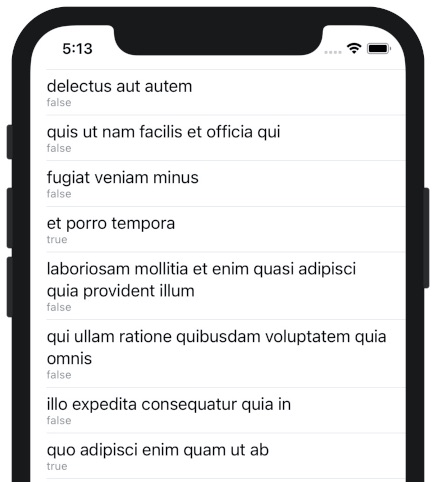
\includegraphics[width=300]{images/json-1.jpg}
\label{fig:JSON-1}
\end{center}
\end{enumerate}
\subsection{Demo 2}
\label{sec:orgaceddd1}
\begin{enumerate}
\item MVVM
\label{sec:orgd6c6968}
\begin{itemize}
\item Model: FlowModel.swift\\
\item View: ContentView.swift\\
\item ViewModel: Flow.swift\\
\end{itemize}
\item FlowModel.swift
\label{sec:org72d5cec}
\lstset{breaklines=true,language=swift,label= ,caption= ,captionpos=b,firstnumber=1,numbers=left}
\begin{lstlisting}
import Foundation

struct FlowModel: Decodable, Hashable {
    var 年: Int? = nil
    var 月: Int? = nil
    var 總運量: Int? = nil
    var 日均運量: Int? = nil
    var 假日均運量: Int? = nil
    var 月台上刷卡日均筆數: Double? = nil
    var 車上刷卡日均筆數: Double? = nil
    var 售票機日均筆數: Double? = nil
    var 補票日均筆數: Double? = nil
    var 團體票日均筆數: Double? = nil
}
\end{lstlisting}
\item ContentView.swift
\label{sec:org0e481c1}
\lstset{breaklines=true,language=swift,label= ,caption= ,captionpos=b,firstnumber=1,numbers=left}
\begin{lstlisting}
import SwiftUI

struct ContentView: View {
    @ObservedObject var flow = FetchFlow()

    var body: some View {
        NavigationView {
            List() {
                ForEach(flow.flows, id: \.self) {(item) in
                    NavigationLink(destination: Text("總運量: \(item.總運量!)")) {
                        HStack {
                            Text("\(item.年!)年\(item.月!)月")
                            Text("\(item.日均運量!)")
                        }
                    }
                }
            }.navigationTitle("")
        }
    }
}
struct ContentView_Previews: PreviewProvider {
    static var previews: some View {
        ContentView()
    }
}

\end{lstlisting}
\item Flow.swift
\label{sec:org23221ee}
\lstset{breaklines=true,language=swift,label= ,caption= ,captionpos=b,firstnumber=1,numbers=left}
\begin{lstlisting}
import Foundation
class FetchFlow: ObservableObject {
    @Published var flows = [FlowModel]()
    init() {
        let urlstr = "https://data.kcg.gov.tw/dataset/6f29f6f4-2549-4473-aa90-bf60d10895dc/resource/30dfc2cf-17b5-4a40-8bb7-c511ea166bd3/download/lightrailtraffic.json"
        guard let url = URL(string: urlstr) else {
            print("Invalid json url")
            return
        }
        URLSession.shared.dataTask(with: url) {(data, response, error) in
            do {
                if let flowData = data {
                    let decodeData = try JSONDecoder().decode([FlowModel].self, from: flowData)

                    DispatchQueue.main.async {
                        self.flows = decodeData
                    }
                } else {
                    print("No data")
                }
            } catch {
                print("\(error)")
            }
        }.resume()
    }
}
\end{lstlisting}
\item Result
\label{sec:orgfb8159b}
\begin{center}
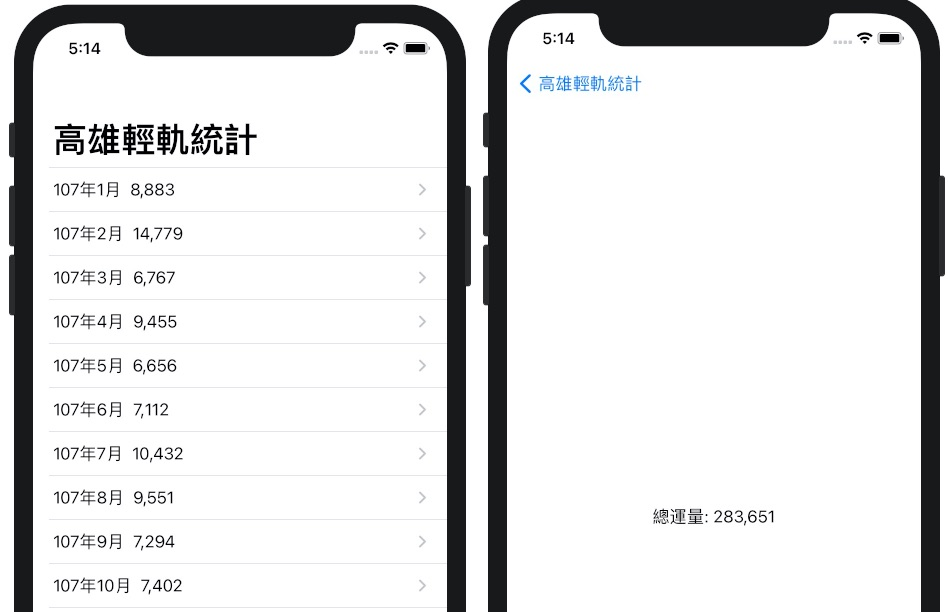
\includegraphics[width=500]{images/json-2.jpg}
\label{fig:JSON-2}
\end{center}
\end{enumerate}
\subsection{公開資料平台}
\label{sec:org303fd58}
\begin{itemize}
\item \href{https://data.gov.tw/}{政府資料開放平台}\\
\item \href{https://data.kcg.gov.tw/dataset}{高雄市政府開放資料集}\\
\item \href{https://data.tainan.gov.tw/dataset}{台南市政府開放資料集}\\
\item \href{https://ptx.transportdata.tw/PTX/Service}{公共運輸整合資訊}\\
\item \href{https://kaleidosblog.s3-eu-west-1.amazonaws.com/json/tutorial.json}{country/code JSON sample}\\
\end{itemize}
\subsection{Further Reading}
\label{sec:org1b12cfa}
\begin{itemize}
\item \href{https://www.youtube.com/watch?v=HvfE4G9PfeU}{SwiftUI Tutorial - Using an API and Decoding JSON Data}\\
\item \href{https://www.youtube.com/watch?v=tdxKIPpPDAI}{iOS Swift Tutorial: Use Web APIs and JSON Data with Swift 5}- \href{https://www.ioscreator.com/tutorials/swiftui-json-list-tutorial}{SwiftUI Fetch JSON Data into List}\\
\item \href{https://programmingwithswift.com/parse-json-from-file-and-url-with-swift/}{Parse JSON from file and URL with Swift}\\
\item \href{https://www.youtube.com/watch?v=1en4JyW3XSI}{Making an API call and fetch JSON data in SwiftUI}\\
\item \href{https://benoitpasquier.com/encoding-decoding-json-swift4/}{The best way to encode and decode JSON in Swift4 }\\
\item \href{https://www.reddit.com/r/swift/comments/emw0i3/jsondecoder\_fails\_if\_i\_dont\_have\_an\_id\_for\_each/}{JSONDecoder fails if I don't have an ``id'' for each item\ldots{} why doesn't UUID work?}\\
\item \href{https://medium.com/\%E5\%BD\%BC\%E5\%BE\%97\%E6\%BD\%98\%E7\%9A\%84-swift-ios-app-\%E9\%96\%8B\%E7\%99\%BC\%E6\%95\%99\%E5\%AE\%A4/\%E8\%A7\%A3\%E6\%B1\%BAjson-key\%E4\%B8\%8D\%E5\%9B\%BA\%E5\%AE\%9A\%E6\%99\%82\%E5\%87\%BA\%E7\%8F\%BE-no-value-associated-with-key-codingkeys-\%E7\%8B\%80\%E6\%B3\%81-720d7d09486a}{解決Json Key不固定時出現“No value associated with key CodingKeys” 狀況}\\
\end{itemize}
\newpage

\section{Protocols}
\label{SW-Protocols}
\begin{itemize}
\item Protocols are a fundamental feature of Swift. They play a leading role in the structure of the Swift standard library and are a common method of abstraction. They provide a similar experience to interfaces that some other languages have. An advantage of protocols in Swift is that objects can conform to multiple protocols.\footnote{\href{https://www.raywenderlich.com/6742901-protocol-oriented-programming-tutorial-in-swift-5-1-getting-started}{Protocol-Oriented Programming Tutorial in Swift 5.1: Getting Started}\\}\\
\item Protocol 是一個只宣告不定義的型別,然而這個特性可以讓我們的程式更有彈性,像在 IOS SDK 裡面,耳熟能詳的 Delegate,就大量的運用 Potocol,方便我們客製化事件發生時要處理的事情。\footnote{\href{https://medium.com/\%E5\%BD\%BC\%E5\%BE\%97\%E6\%BD\%98\%E7\%9A\%84-swift-ios-app-\%E9\%96\%8B\%E7\%99\%BC\%E6\%95\%99\%E5\%AE\%A4/\%E7\%B0\%A1\%E6\%98\%93\%E8\%AA\%AA\%E6\%98\%8Eswift-4-protocol-919b7f9cbaee}{『簡易說明Swift 4』Protocol}\\}\\

\item 對任何程式開發來說,減少重覆的 code,把權責明確分開,讓 code 維護性變好,是非常重要的課題。而在現今的軟體開發模式中,有許多方法可以做到這點,最為人所知的一個模式,就是利用繼承 (Inheritance),把會重覆利用的部份放在母類別,讓其它子類別去繼承。另外一種做法,則是利用 Composition Pattern,將功能做成組件分出來,讓需要的模組去組合取用。\footnote{\href{https://www.appcoda.com.tw/protocol-extension/}{利用 Protocol Extension 減少重覆的 Code 大大增強 Code 的維護性}\\}\\
\end{itemize}
\begin{verse}
A protocol defines a blueprint of methods, properties, and other requirements that suit a particular task or piece of functionality. The protocol can then be adopted by a class, structure, or enumeration to provide an actual implementation of those requirements. Any type that satisfies the requirements of a protocol is said to conform to that protocol. \footnote{\href{https://docs.swift.org/swift-book/LanguageGuide/Protocols.html}{Protocols}\\}\\
\end{verse}

\begin{itemize}
\item 協定提供類型可以做的資訊,Classes 和 structs 則提供物件的資訊,協定則提供物件將會執行的動作。\footnote{\href{https://www.appcoda.com.tw/swift-protocol/}{Swift開發指南:Protocols與Protocol Extensions的使用心法}\\\label{orgeca31e4}}\\
\end{itemize}
\begin{verse}
協定是 Swift 一個重要的特性,它會定義出為了完成某項任務或功能所需的方法、屬性,但是本身不會實作這些任務跟功能,而僅僅只是表達出該任務或功能的名稱。協定為方法、屬性、以及其他特定的任務需求或功能定義藍圖。協定可被 class、struct、或 enum 類型採納以提供所需功能的具體實現。滿足了協定中需求的任意類型都叫做遵循了該協定。\\
\end{verse}

除了指定遵循類型必須實現的要求外,你可以擴展一個協定以實現其中的一些需求或實現一個符合類型的可以利用的附加功能。\footnote{\href{https://ithelp.ithome.com.tw/articles/10197366}{Day-29 Swift 語法(25) - 協定 Protocol}\\}\\
\begin{itemize}
\item 例如,你可能有一個名為 str 的變量,其類型為 String。身為一個開發人員,你應該知道 str 代表 String,如果我們定義了一個名為 StringProtocol 的協定,它具有所有的 String 的 API,我們可以擴展任何類型去遵循 StringProtocol(意思是滿足其所有要求),如此一來,即可以使用該對象,讓它就像是一個 String,儘管我們不知道它是什麼!如果看起來像一隻鴨子,游泳像一隻鴨子,叫聲像一隻鴨子,那就是一隻鴨子。我們新的 StringProtocol 可以告訴那些遵守它協定的類型能夠做什麼,且不需要知道這些類型的資訊。\textsuperscript{\ref{orgeca31e4}}\\
\end{itemize}
\subsection{Protocol Syntax}
\label{sec:orgb26859a}
\begin{enumerate}
\item Syntax
\label{sec:orgae4ed44}
\lstset{breaklines=true,language=swift,label= ,caption= ,captionpos=b,firstnumber=1,numbers=left}
\begin{lstlisting}
protocol SomeProtocol {
    // protocol definition goes here
}
\end{lstlisting}
Classes , structs, enums can adopt these protocol by placing protocol’s name after the type’s name, separated by a colon, as part of their definition. Multiple protocols can be listed, and are separated by commas:\footnote{\href{https://abhimuralidharan.medium.com/all-about-protocols-in-swift-11a72d6ea354}{All about protocols in swift}\\}\\
\lstset{breaklines=true,language=swift,label= ,caption= ,captionpos=b,firstnumber=1,numbers=left}
\begin{lstlisting}
struct SomeStructure: FirstProtocol, AnotherProtocol {
    //structure definition goes here
}
\end{lstlisting}
\item DEMO
\label{sec:orgcd269a0}
\lstset{breaklines=true,language=swift,label= ,caption= ,captionpos=b,firstnumber=1,numbers=left}
\begin{lstlisting}
protocol Polite {
    func sayHello()
}

struct Teacher: Polite {
    var name: String
    func sayHello() {
        print("同學好")
    }
}

struct Student: Polite {
    var name: String
    func sayHEllo() {
        print("老師好")
    }
}

var aPolitePerson: Polite = Teacher()
aPolitePerson.name = "Mr. Yen"
aPolitePerson.sayHellow()
aPolitePerson = Student()
aPolitePerson.sayHello()
\end{lstlisting}
\item Adding property requirements
\label{sec:org069cb1c}
source: \href{https://abhimuralidharan.medium.com/all-about-protocols-in-swift-11a72d6ea354}{All about protocols in swift}\\
\begin{itemize}
\item A protocol can have properties as well as methods that a class, enum or struct conforming to this protocol can implement.\\
\item A protocol declaration only specifies the required property name and type. It doesn’t say anything about whether the property should be a stored one or a computed one.\\
\item A protocol also specifies whether each property must be gettable or gettable and settable.\\
\item Property requirements are always declared as variable properties, prefixed with the var keyword.\\
\item Gettable and settable properties are indicated by writing \{ get set \} after their type declaration, and gettable properties are indicated by writing \{ get \}.\\
\end{itemize}
\lstset{breaklines=true,language=swift,label= ,caption= ,captionpos=b,firstnumber=1,numbers=left}
\begin{lstlisting}
protocol SomeProtocol {
    var mustBeSettable: Int { get set }
    var doesNotNeedToBeSettable: Int { get }
}
\end{lstlisting}
\item Protocols with mutating methods
\label{sec:org95daf92}
Mutating methods are methods that we use on value types like structs and enums. These methods are allowed to modify the instance it belongs to and any properties of that instance. A small example:\\

Consider a simple struct Rectangle:\\
\lstset{breaklines=true,language=swift,label= ,caption= ,captionpos=b,firstnumber=1,numbers=left}
\begin{lstlisting}
struct Rectangle {
    var width = 1
    var height = 1

    func area() -> Int {
        return width * height
    }

    mutating func scaleBy(value: Int) {
        width *= value
        height *= value
    }
}
\end{lstlisting}
The scaleBy(value:) method modifies the value of width and height. So it should be marked as mutating. Otherwise the compiler will throw error at you.\\

\begin{verse}
If you mark a protocol instance method requirement as mutating, you do not need to write the mutatingkeyword when writing an implementation of that method for a class. The mutating keyword is only used by structures and enumerations.\\
\end{verse}
Consider an enum and class implementing a protocol with mutating function:\\
\lstset{breaklines=true,language=swift,label= ,caption= ,captionpos=b,firstnumber=1,numbers=left}
\begin{lstlisting}
protocol Togglable {
    mutating func toggle()
}

enum OnOffSwitch: Toggglable {
    case off, on
    mutating func toggle() {
        switch self {
        case .off:
            self = .on
        case .on:
            self = .off
        }
    }
}

var lightSwitch = OnOffSwitch.off
lightSwitch.toggle()

class ToggleClass: Togglable {
    var someBool = false
    func toggle() {
        someBool = true
    }
}

let toggleClassObj = ToggleClass()
toggleClassObj.toggle()
\end{lstlisting}
\item Initializer Requirements
\label{sec:org9c66597}
Protocols can have specific initializers like normal methods which the conforming types can implement.\\
\lstset{breaklines=true,language=swift,label= ,caption= ,captionpos=b,firstnumber=1,numbers=left}
\begin{lstlisting}
protocol SomeProtocol {
    init(someParameter: Int)
}
\end{lstlisting}
\end{enumerate}
\subsection{DEMO}
\label{sec:org8be615d}
\lstset{breaklines=true,language=swift,label= ,caption= ,captionpos=b,firstnumber=1,numbers=left}
\begin{lstlisting}
protocol Sound {
    func makeSound()
}

struct Dog: Sound {
    func makeSound() {
        print("Woof")
    }
}

struct Tree: Sound {
    func makeSound() {
        print("Susrrate")
    }
}

struct iPhone: Sound {
    func makeSound() {
        print("Ring")
    }
}
\end{lstlisting}
\subsection{範例}
\label{sec:orgc445a74}
\begin{enumerate}
\item 版本 1
\label{sec:org25f2d0b}
本例中有兩個 struct: Song, Album 以及一個 class 用來播放 Song 或 Album,原本的 Player 要為不同的 struct 寫不同的 func,而且程式碼大多重複。\\
\lstset{breaklines=true,language=swift,label= ,caption= ,captionpos=b,firstnumber=1,numbers=left}
\begin{lstlisting}
import Cocoa
import AVKit

struct Song {
    var name: String
    var album: Album
    var audioURL: URL
    var isLiked: Bool
}

struct Album {
    var name: String
    var imageURL: URL
    var audioURL: URL
    var isLiked: Bool
}

class Player {
    private let avPlayer = AVPlayer()

    func play(_ song: Song) {
        let item = AVPlayerItem(url: song.audioURL)
        avPlayer.replaceCurrentItem(with: item)
        avPlayer.play()
    }

    func play(_ album: Album) {
        let item = AVPlayerItem(url: album.audioURL)
        avPlayer.replaceCurrentItem(with: item)
        avPlayer.play()
    }
}
\end{lstlisting}
\item 版本 2
\label{sec:org5508995}
宣告一個 protocol,定義 audioURL 變數(read only),然後令兩個 struct 皆遵循該 protocol(方式有二),如此,原本的 Player class 中的 play func 就能只寫一次。\\
\lstset{breaklines=true,language=swift,label= ,caption= ,captionpos=b,firstnumber=1,numbers=left}
\begin{lstlisting}
import Cocoa
import AVKit

protocol Playable {
    var audioURL: URL { get }
}

struct Song: Playable {
    var name: String
    var album: Album
    var audioURL: URL
    var isLiked: Bool
}

struct Album {
    var name: String
    var imageURL: URL
    var audioURL: URL
    var isLiked: Bool
}

extension Album: Playable {}
class Player {
    private let avPlayer = AVPlayer()

    func play(_ resource: Playable) {
        let item = AVPlayerItem(url: resource.audioURL)
        avPlayer.replaceCurrentItem(with: item)
        avPlayer.play()
    }
}
\end{lstlisting}
\item 版本 3
\label{sec:orge42dd0b}
原本 protocol 的真正意思其實只是在確定 audioURL 是否能正確轉換成 Audio,所以其實將 protocol name 由 Playable 改為 AudioURLConvertable 會更貼近事實。\\
\lstset{breaklines=true,language=swift,label= ,caption= ,captionpos=b,firstnumber=1,numbers=left}
\begin{lstlisting}
import Cocoa
import AVKit

protocol AudioURLConvertable {
    var audioURL: URL { get }
}

struct Song: AudioURLConvertable {
    var name: String
    var album: Album
    var audioURL: URL
    var isLiked: Bool
}

struct Album: AudioURLConvertable {
    var name: String
    var imageURL: URL
    var audioURL: URL
    var isLiked: Bool
}

class Player {
    private let avPlayer = AVPlayer()

    func play(_ resource: AudioURLConvertable) {
        let item = AVPlayerItem(url: resource.audioURL)
        avPlayer.replaceCurrentItem(with: item)
        avPlayer.play()
    }
}

\end{lstlisting}
\end{enumerate}
\subsection{mutating}
\label{sec:org6fe9015}
protocol 除了可以提供傳回值型態的彈性,也可以用來變更 class/struct 中的屬性。如:\\
\lstset{breaklines=true,language=swift,label= ,caption= ,captionpos=b,firstnumber=1,numbers=left}
\begin{lstlisting}
import Cocoa
import AVKit

protocol Likeable {
    mutating func markAsLiked()
}

struct Song {
    var name: String
    var album: Album
    var audioURL: URL
    var isLiked: Bool
}

struct Album {
    var name: String
    var imageURL: URL
    var audioURL: URL
    var isLiked: Bool
}

extension Song: Likeable {
    mutating func markAsLiked() {
        isLiked = true
    }
}
\end{lstlisting}
可以在不改變原 struct Album 的情況下,藉由 extension 來擴充 Song,使其遵循 Likeable protocol,提供變供屬性 isLiked 的值,*這在擴充 API 功能時特別有用*。\\
\subsection{擴充 protocol}
\label{sec:orgdb1e97a}
除了擴充現有 struct,protocol 也可以用來擴充 protocol,如:\\
\lstset{breaklines=true,language=swift,label= ,caption= ,captionpos=b,firstnumber=1,numbers=left}
\begin{lstlisting}
import Cocoa
import AVKit

protocol Likeable {
    var isLiked: Bool {get set}
}

extension Likeable {
    mutating func markAsLiked() {
        isLiked = true
    }
}

struct Song {
    var name: String
    var album: Album
    var audioURL: URL
    var isLiked: Bool
}

struct Album {
    var name: String
    var imageURL: URL
    var audioURL: URL
    var isLiked: Bool
}

extension Song: Likeable {}
extension Album: Likeable {}
\end{lstlisting}
\subsection{Further Reading}
\label{sec:org99a45d3}
\begin{itemize}
\item \href{https://docs.swift.org/swift-book/LanguageGuide/Protocols.html}{Protocol}\\
\item \href{https://appcoda.com.tw/swift-protocol/}{Swift開發指南:Protocols與Protocol Extensions的使用心法}\\
\item \href{https://abhimuralidharan.medium.com/all-about-protocols-in-swift-11a72d6ea354}{All about protocols in SWIFT}\\
\item \href{https://blog.csdn.net/XunCiy/article/details/107367571}{Swift5 14.Protocols}\\
\end{itemize}

\newpage

\section{Enum}
\label{SW-enum}
enumerations(或稱為enums)是Swift中一種特殊類型,它允許你表示多個「情況」或可能性。Enums(列舉)類似於Bool,但Bool只能是true或false,enums可以由開發者自行定義各種情況\footnote{\href{https://appcoda.com.tw/mastering-swift/}{精通Swift:列舉、閉包、泛型、Protocols和高階函數}\\}\\

\subsection{without enum}
\label{sec:org786e6b8}
假設我們要登錄學生的學習等第(A, B, C, D, E, F),如下\\
\lstset{breaklines=true,language=swift,label= ,caption= ,captionpos=b,firstnumber=1,numbers=left}
\begin{lstlisting}
var Tom = "A"
var John = "B"
var James = "I" //Error
print(James)
\end{lstlisting}

上述程式中的James其等第明顯超出合理範圍,對於後續要進行的判斷可能會出現很大問題,此時便是enum適用時機\\

\subsection{with enum}
\label{sec:org5ee97fc}
\lstset{breaklines=true,language=swift,label= ,caption= ,captionpos=b,firstnumber=1,numbers=left}
\begin{lstlisting}
enum grade {
    case A
    case B
    case C
    case D
    case E
    case F
}

var Tome = grade.A
var John = grade.B
var James = grade.C
\end{lstlisting}
判斷檔案下載結果為另一項典型的enum適用情境:\\
\lstset{breaklines=true,language=swift,label= ,caption= ,captionpos=b,firstnumber=1,numbers=left}
\begin{lstlisting}
enum DownloadStatus {
    case downloading
    case finished
    case failed
    case cancelled
}
var currentStatus = DownloadStatus.downloading
\end{lstlisting}
\subsection{enum的rawValue}
\label{sec:org48270b1}

配合rawValue定義enum的值,可以讓enum自帶有意義的資訊。\footnote{\href{https://hugolu.gitbooks.io/learn-swift/content/Advanced/Enum.html}{Swift學習筆記 }\\}\\
\lstset{breaklines=true,language=swift,label= ,caption= ,captionpos=b,firstnumber=1,numbers=left}
\begin{lstlisting}
enum Pet: String {
    case Dog = "🐶"
    case Cat = "🐱"
    case Rabbit = "R"
}

var myPet = Pet.Rabbit
print("my pet is a \(myPet.rawValue)")    //output: my pet is a 🐰
\end{lstlisting}

\begin{verbatim}
my pet is a R
\end{verbatim}
\subsection{enum v.s. switch}
\label{sec:org5322659}
enum最大的用處就是搭配switch。\\
\lstset{breaklines=true,language=swift,label= ,caption= ,captionpos=b,firstnumber=1,numbers=left}
\begin{lstlisting}
let currentStatus = DownloadStatus.downloading

switch currentStatus {
case .downloading:
    print("Downloading...")

case .finished:
    print("Just finished the download...")

case .failed:
    print("Failed to download the file...")

case .cancelled:
    print("The download is cancelled...")
}
\end{lstlisting}

\subsection{Swift列舉中最強大的功能之一:associated values}
\label{sec:orgd7a9fb4}
associated values。它允許我們在列舉中儲存額外的數據。我們宣告一個新的列舉,稱為WeatherCondition,它讓我們在每個天氣條件中可額外挾帶一些資訊:\\
\lstset{breaklines=true,language=swift,label= ,caption= ,captionpos=b,firstnumber=1,numbers=left}
\begin{lstlisting}
enum Cloud {
    case cirrus
    case cumulus
    case altocumulus
    case stratus
    case cumulonimbus
}

enum WeatherCondition {
    case sunny(temperature: Float)
    case rainy(inchesPerHour: Float)
    case cloudy(cloudType: Cloud, windSpeed: Float)
}
\end{lstlisting}
WeatherCondition的宣告。我們提供三個情境,在enum每個情境中都存有附加資訊。在sunny情況下,儲存一個參數名稱為temperature的Float。在rainy情況下,附帶一個Float類型的參數,命名為inchesPerHour,另外在cloudy情況下,我們附帶兩個參數,分別為Cloud類型的cloudType和Float類型的windSpeed。\\
\lstset{breaklines=true,language=swift,label= ,caption= ,captionpos=b,firstnumber=1,numbers=left}
\begin{lstlisting}
let currentWeather = WeatherCondition.cloudy(cloudType: .cirrus, windSpeed: 4.2)

switch currentWeather {
case .sunny(let temperature):
    print("It is sunny and the temperature is \(temperature).")

case .rainy(let inchesPerHour):
    print("It is raining at a rate of \(inchesPerHour) inches per hour.")

case .cloudy(let cloudType, let windSpeed):
    print("It is cloudy; there are \(cloudType) clouds in the sky, and the wind speed is \(windSpeed).")
}
\end{lstlisting}

\section{Struct v.s. Class}
\label{sec:orgfcc22b5}
\href{https://www.hackingwithswift.com/books/ios-swiftui/why-does-swiftui-use-structs-for-views}{資料來源:Why does SwiftUI use structs for views?}\\
If you ever programmed for UIKit or AppKit (Apple’s original user interface frameworks for iOS and macOS) you’ll know that they use classes for views rather than structs. SwiftUI does not: we prefer to use structs for views across the board, and there are a couple of reasons why.\footnote{\href{https://www.hackingwithswift.com/books/ios-swiftui/why-does-swiftui-use-structs-for-views}{Why does SwiftUI use structs for views?}\\}\\
\begin{itemize}
\item Structs are simpler and faster than classes.\\
In SwiftUI, all our views are trivial structs and are almost free to create. Think about it: if you make a struct that holds a single integer, the entire size of your struct is… that one integer. Nothing else. No surprise extra values inherited from parent classes, or grandparent classes, or great-grandparent classes, etc – they contain exactly what you can see and nothing more.\\

\item You can see this in action when you look at the kinds of things that can be a view. We already used Color.red and LinearGradient as views – trivial types that hold very little data. In fact, you can’t get a great deal simpler than using Color.red as a view: it holds no information other than “fill my space with red”.\\

\item In comparison, Apple’s documentation for UIView lists about 200 properties and methods that UIView has, all of which get passed on to its subclasses whether they need them or not.\\
\end{itemize}
\subsection{What is in class/struct}
\label{sec:org4dbee0d}
\href{https://www.avanderlee.com/swift/struct-class-differences/}{資料來源:Struct vs classes in Swift: The differences explained}\\
\begin{enumerate}
\item What is a class in Swift?
\label{sec:orgb5c2613}
A class in Swift is a reference type which can contain:\\
\begin{itemize}
\item properties\\
\item methods\\
\item subscripts\\
\item initializers\\
\item protocol conformances\\
\item extensions\\
\end{itemize}

It’s often described as a template definition of an object, like in the following Article instance definition:\\
\lstset{breaklines=true,language=swift,label= ,caption= ,captionpos=b,firstnumber=1,numbers=left}
\begin{lstlisting}
class ArticleClass {
    let title: String
    let url: URL
    var readCount: Int = 0

    init(title: String, url: URL) {
        self.title = title
        self.url = url
    }
}
\end{lstlisting}
\item What is a struct in Swift?
\label{sec:orge99f27d}
A struct in Swift is a value type which, just like classes, can contain:\\
\begin{itemize}
\item properties\\
\item methods\\
\item subscripts\\
\item initializers\\
\item protocol conformances\\
\item extensions\\
\end{itemize}

It can also be seen as a template definition of an object, like in the following Article instance definition:\\
\lstset{breaklines=true,language=swift,label= ,caption= ,captionpos=b,firstnumber=1,numbers=left}
\begin{lstlisting}
struct ArticleStruct {
    let title: String
    let url: URL
    var readCount: Int = 0
}
\end{lstlisting}
\item What are the differences between a struct and a class?
\label{sec:orgf14f346}
\url{images/coffee.gif}\\
When you pass a class object around your program, you are actually passing a reference to that object, so different parts of your program can share and modify your object. When you pass a structure [ or enum] around your program, what gets passes around is a copy of the structure. So modifications to structures don’t get shared.\footnote{\href{https://abhimuralidharan.medium.com/difference-between-a-struct-and-a-class-in-swift-53e08df73714}{Difference between a struct and a class in Swift}\\\label{orged9f2cf}}\\

One of the major benefits of value types is that they are thread-safe not requiring any\\
 synchronization.\textsuperscript{\ref{orged9f2cf}} Structs always have unique owners, whereas with classes multiple things can point to the same value.\footnote{\href{https://www.hackingwithswift.com/books/ios-swiftui/why-state-only-works-with-structs}{Why @State only works with structs}\\\label{org8e274cf}}\\

Classes don’t need the \textbf{mutating} keyword before methods that change their properties, because you can change properties of constant classes.\\
In practice, what this means is that if we have two SwiftUI views and we send them both the same struct to work with, they actually each have a unique copy of that struct; if one changes it, the other won’t see that change. On the other hand, if we create an instance of a class and send that to both views, they will share changes.\textsuperscript{\ref{org8e274cf}}\\
Value vs reference types\\

One of the most important differences is that a struct is a value type while a class is a reference type. References to a class instance share single data which means that any changes in that class will be available to each reference.\\

\lstset{breaklines=true,language=swift,label= ,caption= ,captionpos=b,firstnumber=1,numbers=left}
\begin{lstlisting}
let articleClass = ArticleClass(title: "Struct vs Class", url: URL(string: "www.avanderlee.com")!)
let articleClassCopy = articleClass

articleClass.readCount = 10
print(articleClassCopy.readCount) // Prints: 10
\end{lstlisting}

A struct is a value type and will create a unique copy for each new reference.\\
\lstset{breaklines=true,language=swift,label= ,caption= ,captionpos=b,firstnumber=1,numbers=left}
\begin{lstlisting}
var articleStruct = ArticleStruct(title: "Struct vs Class", url: URL(string: "www.avanderlee.com")!, readCount: 0)
var articleStructCopy = articleStruct

articleStruct.readCount = 10
print(articleStructCopy.readCount) // Prints: 0
\end{lstlisting}
\begin{enumerate}
\item The benefit of mutation in safety
\label{sec:orgbd211f4}
With this, structs have the benefit of mutation in safety as you can trust that no other part of your app is changing the data at the same time. This makes it easier to reason about your code and is especially helpful in multi-threaded environments where a different thread could alter your data at the same time.\\
\item Structs get an initializer for free
\label{sec:org7573e76}
If you go back and compare the above code examples you can see that the ArticleClass has a defined initializer which is required for classes. Structs, however, get an initializer for free.\\
\lstset{breaklines=true,language=swift,label= ,caption= ,captionpos=b,firstnumber=1,numbers=left}
\begin{lstlisting}
// Before Swift 5.1 Memberwise initializers:
// Generated memberwise init: init(title: String, url: URL, readCount: Int)
let article = ArticleStruct(title: "", url: URL(string: "")!, readCount: 0)

// After Swift 5.1 Memberwise initializers, using the default 0 for read count
// Generated memberwise init: init(title: String, url: URL, readCount: Int = 0)
let article = ArticleStruct(title: "", url: URL(string: "")!)
\end{lstlisting}
\item Classes allow inheritance
\label{sec:org7fb7720}
Classes can inherit the characteristics of another class and with that, act like abstract classes. A common example is a custom view controller which inherit from UIViewController.\\

With protocols in Swift, this is often no longer needed and replaceable with protocols. Protocols can be used with both classes and structs while inheritance is only possible with classes.\\
Classes can be deinitialized\\

A class allows executing code just before it gets destroyed by using a deinit method. When you define the same deinit method in a struct you’ll get the following error:\\
\begin{verse}
Deinitializers may only be declared within a class\\
\end{verse}
\end{enumerate}
\end{enumerate}
\subsection{如何決擇? / When should I go for a struct and when for a class?}
\label{sec:org8112fca}
A simple bullet point list will make it a lot easier to decide.\\
\begin{enumerate}
\item You should use a class when:
\label{sec:org7310f90}
\begin{itemize}
\item Comparing instance identity is needed by using \texttt{=}\\
\item Shared mutable state is required\\
\item Objective-C interoperability is required\\
\end{itemize}
\item You should use a struct when:
\label{sec:orgd3b118b}
\begin{itemize}
\item Comparing instance data is needed by using ==\\
\item Unique copies with an independent state are required\\
\item The data is used in multiple threads\\
\end{itemize}
\item Try to go for a struct by default.
\label{sec:orgf91cf98}
Structs make your code easier to reason about and make it easier to work in multithreaded environments which we often have while developing in Swift.\\
\end{enumerate}
\subsection{DEMO}
\label{sec:org43ef412}
以下這個 View 可正常運作,於 TextField 中所做的編輯修改都會即時顯示於 Text 中。\\
\lstset{breaklines=true,language=swift,label= ,caption= ,captionpos=b,firstnumber=1,numbers=left}
\begin{lstlisting}
struct User {
    var firstName" = Bilbo"
    var lastName = "Baggins"
}

struct ContentView: View {
    @State private var user = User()

    var body: some View {
        VStack {
            Text("Your name is \(user.firstName) \(user.lastName).")

            TextField("First name", text: $user.firstName)
            TextField("Last name", text: $user.lastName)
        }
    }
}
\end{lstlisting}
但若將 struct 改為 class,雖程式仍可執行,但 Text 中的姓名卻不再隨 TextField 的修改而連動。\\
To fix this, we need to tell SwiftUI when interesting parts of our class have changed. By “interesting parts” I mean parts that should cause SwiftUI to reload any views that are watching our class – it’s possible you might have lots of properties inside your class, but only a few should be exposed to the wider world in this way.\footnote{\href{https://www.hackingwithswift.com/books/ios-swiftui/sharing-swiftui-state-with-observedobject}{Sharing SwiftUI state with @ObservedObject}\\}\\
若要將 struct 改為 class,則程式要改成:\\
\lstset{breaklines=true,language=swift,label= ,caption= ,captionpos=b,firstnumber=1,numbers=left}
\begin{lstlisting}
class User: ObservableObject{
    @Published var firstName = "Bilbo"
    @Published var lastName = "Baggins"
}

struct ContentView: View {
    @ObservedObject var user = User()

    var body: some View {
        VStack {
            Text("Your name is \(user.firstName) \(user.lastName).")

            TextField("First name", text: $user.firstName)
            TextField("Last name", text: $user.lastName)
        }
    }
}
\end{lstlisting}
Our User class has two properties: firstName and lastName. Whenever either of those two changes, we want to notify any views that are watching our class that a change has happened so they can be reloaded. We can do this using the @Published property observer.\\

@Published is more or less half of @State: it tells Swift that whenever either of those two properties changes, it should send an announcement out to any SwiftUI views that are watching that they should reload.\\

How do those views know which classes might send out these notifications? That’s another property wrapper, @ObservedObject, which is the other half of @State – it tells SwiftUI to watch a class for any change announcements.\\

The @ObservedObject property wrapper can only be used on types that conform to the ObservableObject protocol. This protocol has no requirements, and really all it means is “we want other things to be able to monitor this for changes.”\\

As you’ve seen, rather than just using @State to declare local state, we now take three steps:\\

\begin{itemize}
\item Make a class that conforms to the ObservableObject protocol.\\
\item Mark some properties with @Published so that any views using the class get updated when they change.\\
\item Create an instance of our class using the @ObservedObject property wrapper.\\
\end{itemize}

The end result is that we can have our state stored in an external object, and, even better, we can now use that object in multiple views and have them all point to the same values.\\
\newpage

\section{Publihser and Subscriber}
\label{sec:org54043e1}
\subsection{Publisher}
\label{sec:org0e127f2}
Declares that a type can transmit a sequence of values over time.\\
\begin{enumerate}
\item Declaration
\label{sec:orgb4bcc83}
\lstset{breaklines=true,language=swift,label= ,caption= ,captionpos=b,firstnumber=1,numbers=left}
\begin{lstlisting}
protocol Publisher
\end{lstlisting}
\item Overview
\label{sec:orgcb14dd8}
A publisher delivers elements to one or more \href{https://developer.apple.com/documentation/combine/subscriber}{Subscriber} instances. The subscriber’s Input and Failure associated types must match the Output and Failure types declared by the publisher. The publisher implements the receive (subscriber:) method to accept a subscriber.\\
You connect a subscriber to a publisher by calling the publisher’s subscribe(\uline{:) method. After making this call, the publisher invokes the subscriber’s receive(subscription:) method. This gives the subscriber a Subscription instance, which it uses to demand elements from the publisher, and to optionally cancel the subscription. After the subscriber makes an initial demand, the publisher calls receive(}:), possibly asynchronously, to deliver newly-published elements. If the publisher stops publishing, it calls receive(completion:), using a parameter of type Subscribers.Completion to indicate whether publishing completes normally or with an error.\\

\begin{itemize}
\item sink(receiveCompletion:receiveValue:) executes arbitrary closures when it receives a completion signal and each time it receives a new element.\\
\item assign(to:on:) writes each newly-received value to a property identified by a key path on a given instance.\\
\end{itemize}
\end{enumerate}

\section{Combine}
\label{sec:orgfc99d10}
在 2019 年時,Apple 推出了兩套強大的框架分別是 SwiftUI 以及 Combine,而這兩種全新的框架對於開發者來說是一個重大的改動,它也跟以往我們熟悉的編成方式不同,因此要能夠熟悉這兩個新推出的框架也算是一個大挑戰\footnote{\href{https://medium.com/jeremy-xue-s-blog/swift-combine-\%E5\%85\%A5\%E9\%96\%80\%E4\%BB\%8B\%E7\%B4\%B9-333623e21d3d}{Swift — Combine 入門介紹}\\\label{orgd5285ef}}。\\
\subsection{Publisher\textsuperscript{\ref{orgd5285ef}}}
\label{sec:org357fa48}
Combine 框架提供了一個宣告性(declarative)的 Swift API,其用於隨時間推移的值處理,這些值可以表示多種異步事件。Combine 宣告發布者(Publishers)去暴露隨時間變化的值,而訂閱者(Subscribers)去從發布者那裡接收這些值:\\
\begin{itemize}
\item Publisher 協議宣告了一個可以隨時間傳遞序列值的類型。發布者具有運算符(Operators)來從上游發布者那裡獲得的值採取行動,然後重新發布他們。\\
\item 在發布者鏈的結尾,訂閱者在接收元素的時候對其進行操作。發布者只能在訂閱者明確要求時才發出值。如此一來,你的訂閱者程式碼就可以控制從連接的發布者那裡接受事件的速度\\
\end{itemize}
\subsection{Subscriber\textsuperscript{\ref{orgd5285ef}}}
\label{sec:org2267d06}
Combine 提供了兩個內建的訂閱者,這些訂閱者自動匹配其附屬發布者的輸出和失敗類型:\\
\begin{itemize}
\item sink(receiveCompletion:receiveValue:)\\
採用兩個必包。第一個閉包在收到 Subscribers.Completion 時執行,這是一個枚舉,其表示發布者是正常完成還是因為錯誤而失敗。第二個閉包在收到發布者的元素時執行。\\
\item assign(to:on:)\\
使用 key path 來表示屬性立即將其接收到的每個元素分配給給定對象的屬性。\\
\end{itemize}
例如,你可以使用 sink 訂閱者來印出每次發布者完成以及每次收到元素時的 log:\\
\lstset{breaklines=true,language=swift,label= ,caption= ,captionpos=b,firstnumber=1,numbers=left}
\begin{lstlisting}
let sub = NotificationCenter.default
  .publisher(for: UITextField.textDidChangeNotification, object: filterField)
  .sink(receiveCompletion: {print ($0)},
        receiveValue: { print ($0) })
\end{lstlisting}
sink 和 assign 兩種訂閱者都向其發布者請求無限數量的元素。想要控制接收元素的比率,請透過實現 Subscriber 協議來創建自己的訂閱者。\\
如要更改發布者的輸出類型,請添加一個 map(\_:) 運算符,其閉包將返回不同的類型。在這種情況下,你可以將通知的對象獲取為一個 UITextFiled,然後獲取其 text。\\
在發布者產生所需的類型後,將 sink(receiveCompletion:receiveValue:) 替換為 assign(to:on:)。下面的範例獲取從發布者鏈接收到的字串,並將其分配給自定義的 ViewModel 對象的 fillterString :\\
\lstset{breaklines=true,language=swift,label= ,caption= ,captionpos=b,firstnumber=1,numbers=left}
\begin{lstlisting}
let sub = NotificationCenter.default
  .publisher(for: UITextField.textDidChangeNotification, object: filterField)
  .map( { ($0.object as! UITextField).text!) })
  .assign(to: \MyViewModel.filterString, on: myViewModel)
\end{lstlisting}
\subsection{使用操作符自定義發布者\textsuperscript{\ref{orgd5285ef}}}
\label{sec:orge550b6e}
你可以使用執行某些行為的運算符來擴展 Publisher 實例,否則這些操作需要手動進行編碼。你可以使用以下三個方式來使運算符改善此事件處理鏈:\\
\begin{itemize}
\item 可以使用 filter(\_:) 運算符來忽略特定長度下的輸入或是拒絕非字母數字的字,而不是使用在 text filed 中輸入任何內容時更新 ViewModel。\\
\item 如果過濾運算很昂貴(例如:查詢大型數據庫),則可能要等待用戶停止輸入。為此,我們可以使用 debounce(for:scheduler:options:) 運算符可以設置發布者發出事件之前必須經過的最短時間。RunLoop 類為指定以秒或毫秒為單位的延遲時間提供了方便。\\
\item 如果結果更新了 UI,則可以透過調用 receive(on:options:) 方法 callback 回主線程。透過將 RunLoop 類提供的 Scheduler 實例指定為第一個參數,可以告訴 Combine 在主運算循環上調用你的訂閱者。\\
\end{itemize}
結果發布者宣告如下:\\
\lstset{breaklines=true,language=swift,label= ,caption= ,captionpos=b,firstnumber=1,numbers=left}
\begin{lstlisting}
let sub = NotificationCenter.default
  .publisher(for: UITextField.textDidChangeNotification, object: filterField)
  .map( { ($0.object as! UITextField).text!) })
  .filter( {$0.unicodeScalars.allStatisfy({CharacterSet.alphanumerics.contains($0)})} )
  .debounce(for: .milliseconds(500), scheduler: RunLoop.main)
  .receive(on: RunLoop.main)
  .assign(to: \MyViewModel.filterString, on: myViewModel)
\end{lstlisting}
\subsection{需要時取消發布\textsuperscript{\ref{orgd5285ef}}}
\label{sec:orgd61ac1d}
\subsection{Webs, Video}
\label{sec:orgcbb5aa3}
\href{https://www.youtube.com/watch?v=r7ef2W3kevY}{SwiftUI and Combine All The Things}\\
\href{https://www.youtube.com/watch?v=bRpFHqv0tRQ}{SwiftUI 2.0 + Combine - Getting Started (2020)}\\
\href{https://www.youtube.com/watch?v=YJRApch2cc4}{SwiftUI 2.0 \& Combine: Building a Form with Inline Error Validation}\\
\href{https://www.youtube.com/watch?v=IBelvWwZkJw}{SwiftUI Binding} : @Binding, @StateObject, @ObservedObject, @EnvironmentObject\\

\section{{\bfseries\sffamily TODO} some}
\label{some}
\begin{verse}
Adding the keyword some in front of a return type indicates that the return type is opaque. \footnote{\href{https://medium.com/@PhiJay/whats-this-some-in-swiftui-34e2c126d4c4}{What’s this “some” in SwiftUI?}\\}\\
\end{verse}
\subsection{Generics}
\label{sec:org7e90e70}
\begin{enumerate}
\item 問題
\label{sec:org50377fd}
Generics 允許開發者在不同類型中複用你的程式碼,用來解決下列問題:\\
\lstset{breaklines=true,language=swift,label= ,caption= ,captionpos=b,firstnumber=1,numbers=left}
\begin{lstlisting}
func swapInts(_ a: inout Int, _ b: inout Int) {
    let temporaryB = b
    b = a
    a = temporaryB
}

var num1 = 10
var num2 = 20

swapInts(&num1, &num2)
print(num1)   // 20
print(num2)   // 10
\end{lstlisting}
但若想交換字串,則要寫成\\
\lstset{breaklines=true,language=swift,label= ,caption= ,captionpos=b,firstnumber=1,numbers=left}
\begin{lstlisting}
func swapStrings(_ a: inout String, _ b: inout String) {
    let temporaryB = b
    b = a
    a = temporaryB
}
\end{lstlisting}
可以發現除了參數之外,重複的 code 實在太多\\
\item 解決方案
\label{sec:org553ed31}
將固定型態的參數轉為 Generic type\\
\lstset{breaklines=true,language=swift,label= ,caption= ,captionpos=b,firstnumber=1,numbers=left}
\begin{lstlisting}
import Cocoa

func swapTwoValues<T>(_ a: inout T, _ b: inout T) {
    let temporaryA = a
    a = b
    b = temporaryA
}


var num1 = 10
var num2 = 20

swapTwoValues(&num1, &num2)
print(num1)   // 20
print(num2)   // 10
\end{lstlisting}
另一個例子為 Stack 的實作:\\
原本只能儲存 Int 的 Stack 如下,若要儲存字串則要再另行定義。\\
\lstset{breaklines=true,language=swift,label= ,caption= ,captionpos=b,firstnumber=1,numbers=left}
\begin{lstlisting}
struct IntStack {
    var items = [Int]()
    mutating func push(_ item: Int) {
        items.append(item)
    }
    mutating func pop() -> Int {
        return items.removeLast()
    }
}
\end{lstlisting}
改為 Generic type 後可動態變更為整數 stack 或字串 stack,如:\\
\lstset{breaklines=true,language=swift,label= ,caption= ,captionpos=b,firstnumber=1,numbers=left}
\begin{lstlisting}
struct Stack<Element> {
    var items = [Element]()
    mutating func push(_ item: Element) {
        items.append(item)
    }
    mutating func pop() -> Element {
        return items.removeLast()
    }
}

var stackOfStrings = Stack<String>()
stackOfStrings.push("uno")
stackOfStrings.push("dos")
stackOfStrings.push("tres")
stackOfStrings.push("cuatro")
// the stack now contains 4 strings

\end{lstlisting}
\end{enumerate}
\subsection{opaque}
\label{sec:org0150ff9}
帶有不透明(opaque)返回類型的函數或方法,將會隱藏其返回值的類型\footnote{\href{https://medium.com/jeremy-xue-s-blog/swift-\%E7\%A8\%8B\%E5\%BC\%8F\%E8\%AA\%9E\%E8\%A8\%80-opaque-types-600ad5758b91}{Swift 程式語言 — Opaque Types}\\}\\
\newpage

\section{{\bfseries\sffamily TODO} 進階主題}
\label{advanced}
\begin{itemize}
\item \href{https://developer.apple.com/design/human-interface-guidelines/}{Human Interface Guidelines}: Apple 的人機設計界面指南\\
\item \href{https://developer.apple.com/documentation}{Apple Developer Documentation}: Apple 開發者文件\\
\item \href{https://www.appcoda.com.tw/protocol-extension/}{利用 Protocol Extension 減少重覆的 Code 大大增強 Code 的維護性}\\
\item \href{https://appcoda.com.tw/mastering-swift/}{精通Swift:列舉、閉包、泛型、Protocols和高階函數}\\
\end{itemize}
\newpage
\end{document}
